\documentclass[12pt,a4paper]{report}
\usepackage[utf8]{inputenc}
\usepackage[spanish]{babel}
\usepackage{amsmath}
\usepackage{amsfonts}
\usepackage{amssymb}
\usepackage{lmodern}
\usepackage{amsmath}
\usepackage{enumerate}
\usepackage{algorithmic}
\usepackage{algorithm}
\usepackage[left=2cm,right=2cm,top=2cm,bottom=2cm]{geometry}
\usepackage{graphicx}
\usepackage{mathtools}
\usepackage{stackrel}
\renewcommand{\theequation}{\arabic{equation}}
\newcounter{neq}
\providecommand{\abs}[1]{\lvert#1\rvert}
\newcommand{\LINECOMMENT}[1]{\STATE \(\triangleright\) #1}
\newcommand{\RESET}[1]{\STATE Reset: #1}
\def\BState{\State\hskip-\ALG@thistlm}
\newcommand{\QED}{\hfill \textit{\textbf{Q.E.D.}} \vspace{5mm}}
\newcommand{\PROOF}{\vspace{3mm} \textbf{\underline{Proof:}} }
\author{Agustín Curto, agucurto95@gmail.com \\
			  Francisco Nievas, frannievas@gmail.com}
\title{Resumen de teoremas para el final \\ de Lenguajes Formales y Computabilidad}
\date{2017}

\begin{document}
\maketitle
\tableofcontents

\section{Notación y conceptos básicos}

  % Lemma 1: Sin prueba.
  \begin{lemma}
    \par Sea $S \subseteq \omega \times \SIGMA$, entonces $S$ es rectangular si y solo si se cumple la siguiente
    propiedad:

    \[
      \text{Si } (x, \alpha), \; (y, \beta) \in S \Rightarrow (x, \beta) \in S
    \]
  \end{lemma}

  % Lemma 2: Sin prueba.
  \begin{lemma}
    \par La relación $<$ es un orden total estricto sobre $\SIGMA$.
  \end{lemma}

  % Lemma 3: Sin prueba.
  \begin{lemma}
    \par La función $s^{<}: \SIGMA \rightarrow \SIGMA$, definida recursivamente de la siguiente manera:

    \begin{eqnarray}
  		\nonumber s^{<}(\varepsilon) &=& a_{1} \\
  		\nonumber s^{<}(\alpha a_{i}) &=& \alpha a_{i+1} \qquad \text{para } i < n \\
  		\nonumber s^{<}(\alpha a_{n}) &=& s^{<}(\alpha) a_{1}
    \end{eqnarray}

    \par tiene la siguiente propiedad:

    \[
      s^{<}(\alpha) = \min \{\beta \in \SIGMA: \alpha < \beta\}
    \]
  \end{lemma}

  % Corollary 4: Sin prueba.
  \begin{corollary}
    \par $s^{<}$ es inyectiva.
  \end{corollary}

  % Lemma 5: Sin prueba.
  \begin{lemma}
    \par Se tiene que:

    \begin{enumerate}
      \item $s^{<}(\alpha) \neq \varepsilon$, para cada $\alpha \in \SIGMA$.
      \item Si $\alpha \neq \varepsilon$, entonces $\alpha = s^{<}(\beta)$ para algún $\beta$.
      \item Si $S\subseteq \SIGMA \neq \emptyset$, entonces $\exists \alpha \in S$ tal que $\alpha < \beta$, para cada
      $\beta \in S - \{\alpha\}$.
    \end{enumerate}
  \end{lemma}

  % Lemma 6: Sin prueba.
  \begin{lemma}
    \par Tenemos que:

    \[
      \SIGMA = \{\ast^{<}(0), \ast^{<}(1), \dotsc\}
    \]

    \par Mas aún la función $\ast^{<}$ es biyectiva.
  \end{lemma}

  % Lemma 7: Sin prueba.
  \begin{lemma}
    \par Sea $n \geq 1$ fijo, entonces cada $x \geq 1$ se escribe en forma única de la siguiente manera:

    \[
      x = i_{0} n^{0} + \dotsc + i_{k-1} n^{k-1} + i_{k} n^{k}
    \]

    \par con $k\geq 0$ y $1 \leq i_{0}, \dotsc, i_{k-1}, i_{k} \leq n$.
  \end{lemma}

  % Lemma 8: Sin prueba.
  \begin{lemma}
    \par La función $\#^{<}$ es biyectiva.
  \end{lemma}

  % Lemma 9: Sin prueba.
  \begin{lemma}
    \par Las funciones $\#^{<}$ y $\ast^{<}$ son una inversa de la otra.
  \end{lemma}

  % Lemma 10: Sin prueba.
  \begin{lemma}
    \par Si $p, p_{1}, \dotsc, p_{n}$ son números primos y $p$ divide a $p_{1} \dotsc p_{n}$, entonces $p = p_{i}$,
    para algún $i$.
  \end{lemma}

  % Theorem 11: Sin prueba.
  \begin{theorem}
    \par Para cada $x \in \mathbb{N}$, hay una única sucesión $(s_{1}, s_{2}, \dotsc) \in
    \omega^{\left[\mathbb{N}\right]}$ tal que:

    \[
      x = \underset{i=1}{\overset{\infty}{\Pi}} \; pr(i)^{s_{i}}
    \]

    \par Notar que $\underset{i=1}{\overset{\infty}{\Pi}} \; pr(i)^{s_{i}}$ tiene sentido ya que es un producto que solo
    tiene una cantidad finita de factores no iguales a 1.
  \end{theorem}

  % Lemma 12: Sin prueba.
  \begin{lemma}
    \par Las funciones:

    \begin{eqnarray}
    	\nonumber \mathbb{N} &\rightarrow& \omega^{\left[\mathbb{N}\right]} \\
    	\nonumber x &\rightarrow& ((x)_{1}, (x)_{2}, \dotsc) \\
      \nonumber \\
      \nonumber \omega^{\left[\mathbb{N}\right]} &\rightarrow& \mathbb{N} \\
      \nonumber (s_{1}, s_{2}, \dotsc) &\rightarrow& \left\langle s_{1}, s_{2}, \dotsc \right\rangle
  	\end{eqnarray}

    \par son biyecciones una inversa de la otra.
  \end{lemma}

  % Lemma 13: Sin prueba.
  \begin{lemma}
    \par Para cada $x \in \mathbb{N}$:

    \begin{enumerate}
      \item $Lt(x) = 0 \Leftrightarrow x = 1$
      \item $x = \underset{i=1}{\overset{Lt(x)}{\Pi}} \; pr(i)^{(x)_{i}}$
    \end{enumerate}

    \par Cabe destacar entonces que la función $\lambda ix[(x)_{i}]$ tiene dominio igual a $\mathbb{N}^{2}$ y la
    función $\lambda ix[Lt(x)]$ tiene dominio igual a $\mathbb{N}$.
  \end{lemma}

\section{Procedimientos efectivos}

  % Lemma 14
  \begin{lemma}
    \par Sean $S_{1}, S_{2} \subseteq \omega^{n} \times \SIGMA$ conjuntos $\Sigma$-efectivamente enumerables, entonces:

    \begin{enumerate}[a)]
      \item $S_{1} \cup S_{2}$ es $\Sigma$-efectivamente enumerable.
      \item $S_{1} \cap S_{2}$ es $\Sigma$-efectivamente enumerable.
    \end{enumerate}
  \end{lemma}
  \begin{proof}
    \par El caso en el que alguno de los conjuntos es vacío es trivial. Supongamos que $S_{1}, S_{2} \neq \emptyset$ y
    sean $\mathbb{P}_{1}$ y $\mathbb{P}_{2}$ procedimientos que enumeran a $S_{1}$ y $S_{2}$.

    \begin{enumerate}[a)]
      \item El siguiente procedimiento enumera al conjunto $S_{1} \cup S_{2}$:

        \textbf{Si $x$ es par:} realizar $\mathbb{P}_{1}$ partiendo de $x/2$ y dar el elemento de $S_{1}$ obtenido como
        salida.
        \textbf{Si $x$ es impar:} realizar $\mathbb{P}_{2}$ partiendo de $(x-1)/2$ y dar el elemento de $S_{2}$ obtenido
        como salida.

      \item Veamos ahora que $S_{1} \cap S_{2}$ es $\Sigma$-efectivamente enumerable:

        \textbf{Si $S_{1} \cap S_{2} = \emptyset$:} entonces no hay nada que probar.

        \textbf{Si $S_{1} \cap S_{2} \neq \emptyset$:} sea $z_{0}$ un elemento fijo de $S_{1} \cap S_{2}$. Sea
        $\mathbb{P}$ un procedimiento efectivo el cual enumere a $\omega \times \omega$.

        \vspace{3mm}
        \par El siguiente procedimiento enumera al conjunto $S_{1} \cap S_{2}$:

        \textbf{Etapa 1:}
        Realizar $\mathbb{P}$ con dato de entrada $x$, para obtener un par $(x_{1}, x_{2}) \in \omega \times \omega $.

        \textbf{Etapa 2:}
        Realizar $\mathbb{P}_{1}$ con dato de entrada $x_{1}$ para obtener un elemento $z_{1} \in S_{1}$.

        \textbf{Etapa 3:}
        Realizar $\mathbb{P}_{2}$ con dato de entrada $x_{2}$ para obtener un elemento $z_{2} \in S_{2}$.

        \textbf{Etapa 4:}
        Si $z_{1} = z_{2}$, entonces dar como dato de salida $z_{1}$. En caso contrario dar como dato de salida $z_{0}$.
    \end{enumerate}
  \end{proof}

  % Lemma 15
  \begin{lemma}
    \par Si $S \subseteq \omega^{n} \times \SIGMA$ es $\Sigma$-efectivamente computable entonces $S$ es
    $\Sigma$-efectivamente enumerable.
  \end{lemma}
  \begin{proof}
    \par El caso en el que S es vacío es trivial. Supongamos $S \neq \emptyset$. Sea $(\vec{z}, \gamma) \in S$, fijo.
    Recordemos que $\omega^{n} \times \Sigma^{\ast m}$ es $\Sigma$-efectivamente enumerable. Sean:

    \begin{itemize}
      \item $\mathbb{P}_{1}$ un procedimiento efectivo que enumere a $\omega^{n} \times \Sigma^{\ast m}$
      \item $\mathbb{P}_{2}$ un procedimiento efectivo que compute a $\chi_{S}$.
    \end{itemize}

    \par El siguiente procedimiento enumera a $S$:

    \vspace{3mm}
    \textbf{Etapa 1:}
    Realizar $\mathbb{P}_{1}$ con $x$ de entrada para obtener $(\vec{x}, \vec{\alpha}) \in \omega^{n}\times
    \Sigma^{\ast m}$.

    \textbf{Etapa 2:}
    Realizar $\mathbb{P}_{2}$ con $(\vec{x}, \vec{\alpha})$ de entrada para obtener el valor \textit{Booleano} $e$ de
    salida.

    \textbf{Etapa 3:}
    \textbf{Si $e=1$:} dar como dato de salida $(\vec{x}, \vec{\alpha})$.

    $\qquad\qquad\;\;$\textbf{Si $e=0$:} dar como dato de salida $(\vec{z}, \gamma)$.
  \end{proof}

  \pagebreak
  % Theorem 16
  \begin{theorem}
    \par Sea $S \subseteq \omega^{n}\times \SIGMA$. Son equivalentes:

    \begin{enumerate}[a)]
      \item $S$ es $\Sigma$-efectivamente computable.
      \item $S$ y $(\omega^{n}\times \SIGMA)-S$ son $\Sigma$-efectivamente enumerables.
    \end{enumerate}
  \end{theorem}
  \begin{proof}
    \begin{tabular}{|c|}\hline $(a) \Rightarrow (b)$\\\hline\end{tabular} Si $S$ es $\Sigma$-efectivamente computable,
    por el \textbf{Lemma 15} tenemos que $S$ es $\Sigma$-efectivamente enumerable. Notese además que, dado que $S$ es
    $\Sigma$-efectivamente computable, $(\omega^{n} \times \Sigma^{\ast m}) - S$ también lo es, es decir, que aplicando
    nuevamente el \textbf{Lemma 15} tenemos que $(\omega^{n} \times \Sigma^{\ast m})-S$ es
    $\Sigma$-efectivamente enumerable.

    \vspace{3mm}
    \begin{tabular}{|c|}\hline $(b) \Rightarrow (a)$\\\hline\end{tabular} Sean:

    \begin{itemize}
      \item $\mathbb{P}_{1}$ un procedimiento efectivo que enumere a $S$.
      \item $\mathbb{P}_{2}$ un procedimiento efectivo que enumere a $(\omega^{n}\times \Sigma^{\ast m}) - S$.
    \end{itemize}

    \par El siguiente procedimiento computa el predicado $\chi_{S}$:

    \vspace{3mm}
    \textbf{Etapa 1:}
    Darle a la variable $T$ el valor $0$.

    \textbf{Etapa 2:}
    Realizar $\mathbb{P}_{1}$ con el valor de $T$ como entrada para obtener de salida la upla $(\vec{y}, \vec{\beta})$.

    \textbf{Etapa 3:}
    Realizar $\mathbb{P}_{2}$ con el valor de $T$ como entrada para obtener de salida la upla $(\vec{z}, \vec{\gamma})$.

    \textbf{Etapa 4:}
    \textbf{Si $(\vec{y}, \vec{\beta}) = (\vec{x}, \vec{\alpha})$:} entonces detenerse y dar como dato de salida el
    valor $1$.

    $\qquad\qquad\;\;$\textbf{Si $(\vec{z}, \vec{\gamma}) = (\vec{x}, \vec{\alpha})$:} entonces detenerse y dar como
    dato de salida el valor $0$.

    $\qquad\qquad\;\;$\textbf{Si no sucede ninguna de las dos posibilidades:} aumentar en $1$ el valor de

    $\qquad\qquad\;\;$la variable $T$ y dirijirse a la Etapa 2.
  \end{proof}

  % Theorem 17
  \begin{theorem}
    \par Dado $S \subseteq \omega^{n} \times \SIGMA$, son equivalentes:

    \begin{enumerate}
      \item $S$ es $\Sigma$-efectivamente enumerable.
      \item $S = \emptyset$ ó $S = I_{F}$, para alguna $F: \omega \rightarrow \omega^{n} \times \SIGMA$ tal que cada
        $F_{i}$ es $\Sigma$-efectivamente computable.
      \item $S = I_{F}$, para alguna $F:D_{F} \subseteq \omega^{k} \times \Sigma^{\ast l} \rightarrow \omega^{n} \times
        \SIGMA$ tal que cada $F_{i}$ es $\Sigma$-efectivamente computable.
      \item $S = D_{f}$, para alguna función $f$ la cual es $\Sigma$-efectivamente computable.
    \end{enumerate}
  \end{theorem}

\section{Funciones $\Sigma$-recursivas}

  \textbf{\underline{Lemma 18:}} Si \(f,f_{1},...,f_{n+m}\) son \(\Sigma \)-efectivamente computables, entonces \( f\circ (f_{1},...,f_{n+m})\) lo es.

  \PROOF Sean \(\mathbb{P},\mathbb{P}_{1},...,\mathbb{P}_{n+m}\) procedimientos efectivos los cuales computen las funciones \(f,f_{1},...,f_{n+m}\), respectivamente. Usando estos procedimientos es facil definir un procedimiento efectivo el cual compute a \(f\circ (f_{1},...,f_{n+m})\). \(\Box\)

  \textbf{\underline{Lemma 19:}} Si \(f\) y \(g\) son \(\Sigma \)-efectivamente computables, entonces \(R(f,g)\) lo es.

  \PROOF La Proof es dejada al lector. \(\Box\)

  \textbf{\underline{Lemma 20:}} Si \(f\) y cada \(\mathcal{G}_{a}\) son \(\Sigma \)-efectivamente computables, entonces \(R(f,\mathcal{G})\) lo es.

  \PROOF Es dejada al lector con la recomendacion de que haga la Proof para el caso \( \Sigma =\{@,\& \}\) \(\Box\)

  \textbf{\underline{Theorem 21:}} Si \(f\in \mathrm{PR}^{\Sigma }\), entonces \(f\) es \(\Sigma \)-efectivamente computable.

  \PROOF Dejamos al lector la Proof por induccion en \(k\) de que si \(f\in \mathrm{PR} _{k}^{\Sigma }\), entonces \(f\) es \(\Sigma \)-efectivamente computable, la cual sale en forma directa usando los lemas anteriores que garantizan que los constructores de composicion y recursion primitiva preservan la computabilidad efectiva \(\Box\)

  \textbf{\underline{Lemma 22:}}
  (1) \(\varnothing \in \mathrm{PR}^{\varnothing }\).
  (2) \(\lambda xy\left[ x+y\right] \in \mathrm{PR}^{\varnothing }\).
  (3) \(\lambda xy\left[ x.y\right] \in \mathrm{PR}^{\varnothing }\).
  (4) \(\lambda x\left[ x!\right] \in \mathrm{PR}^{\varnothing }\).

  \PROOF (1) Notese que \(\varnothing =Pred\circ C_{0}^{0,0}\in \mathrm{PR} _{1}^{\varnothing }\)

  (2) Notar que

  \(\displaystyle \begin{array}{rcl} \lambda xy\left[ x+y\right] (0,x_{1}) & =& x_{1}=p_{1}^{1,0}(x_{1}) \\ \lambda xy\left[ x+y\right] (t+1,x_{1}) & =& \lambda xy\left[ x+y\right] (t,x_{1})+1 \\ & =& \left( Suc\circ p_{1}^{3,0}\right) \left( \lambda xy\left[ x+y\right] (t,x_{1}),t,x_{1}\right) \end{array} \)

  lo cual implica que \(\lambda xy\left[ x+y\right] =R\left( p_{1}^{1,0},Suc\circ p_{1}^{3,0}\right) \in \mathrm{PR}_{2}^{\varnothing }.\)
  (3) Primero note que

  \(\displaystyle \begin{array}{rcl} C_{0}^{1,0}(0) & =& C_{0}^{0,0}(\Diamond ) \\ C_{0}^{1,0}(t+1) & =& C_{0}^{1,0}(t) \end{array} \)

  lo cual implica que \(C_{0}^{1,0}=R\left( C_{0}^{0,0},p_{1}^{2,0}\right) \in \mathrm{PR}_{1}^{\varnothing }.\) Tambien note que
  \(\displaystyle \lambda tx\left[ t.x\right] =R\left( C_{0}^{1,0},\lambda xy\left[ x+y\right] \circ \left( p_{1}^{3,0},p_{3}^{3,0}\right) \right) , \)

  lo cual por (1) implica que \(\lambda tx\left[ t.x\right] \in \mathrm{PR} _{3}^{\varnothing }\).
  (4) Note que

  \(\displaystyle \begin{array}{rcl} \lambda x\left[ x!\right] (0) & =& 1=C_{1}^{0,0}(\Diamond ) \\ \lambda x\left[ x!\right] (t+1) & =& \lambda x\left[ x!\right] (t).(t+1), \end{array} \)

  lo cual implica que
  \(\displaystyle \lambda x\left[ x!\right] =R\left( C_{1}^{0,0},\lambda xy\left[ x.y\right] \circ \left( p_{1}^{2,0},Suc\circ p_{2}^{2,0}\right) \right) . \)

  Ya que \(C_{1}^{0,0}=\) \(Suc\circ C_{0}^{0,0}\), tenemos que \(C_{1}^{0,0}\in \mathrm{PR}_{1}^{\varnothing }\). Por (2), tenemos que
  \(\displaystyle \lambda xy\left[ x.y\right] \circ \left( p_{1}^{2,0},Suc\circ p_{2}^{2,0}\right) \in \mathrm{PR}_{4}^{\varnothing }, \)

  obteniendo que \(\lambda x\left[ x!\right] \in \mathrm{PR}_{5}^{\varnothing }\). \(\Box\)


  \textbf{\underline{Lemma 23:}} Supongamos \(\Sigma \) es no vacio.
  (a) \(\lambda \alpha \beta \left[ \alpha \beta \right] \in \mathrm{PR} ^{\Sigma }\)
  (b) \(\lambda \alpha \left[ \left\vert \alpha \right\vert \right] \in \mathrm{PR}^{\Sigma }\)

  \PROOF (a) Ya que

  \(\displaystyle \begin{array}{rcl} \lambda \alpha \beta \left[ \alpha \beta \right] (\alpha _{1},\varepsilon ) & =& \alpha _{1}=p_{1}^{0,1}(\alpha _{1}) \\ \lambda \alpha \beta \left[ \alpha \beta \right] (\alpha _{1},\alpha a) & =& d_{a}(\lambda \alpha \beta \left[ \alpha \beta \right] (\alpha _{1},\alpha )),a\in \Sigma \end{array} \)

  tenemos que \(\lambda \alpha \beta \left[ \alpha \beta \right] =R\left( p_{1}^{0,1},\mathcal{G}\right) \), donde \(\mathcal{G}_{a}=d_{a}\circ p_{3}^{0,3}\), para cada \(a\in \Sigma \).
  (b) Ya que

  \(\displaystyle \begin{array}{rcl} \lambda \alpha \left[ \left\vert \alpha \right\vert \right] (\varepsilon ) & =& 0=C_{0}^{0,0}(\Diamond ) \\ \lambda \alpha \left[ \left\vert \alpha \right\vert \right] (\alpha a) & =& \lambda \alpha \left[ \left\vert \alpha \right\vert \right] (\alpha )+1 \end{array} \)

  tenemos que \(\lambda \alpha \left[ \left\vert \alpha \right\vert \right] =R\left( C_{0}^{0,0},\mathcal{G}\right) \), donde \(\mathcal{G}_{a}=\) \( Suc\circ p_{1}^{1,1}\), para cada \(a\in \Sigma .\). \(\Box\)


  \textbf{\underline{Lemma 24:}}
  (a) \(C_{k}^{n,m},C_{\alpha }^{n,m}\in \mathrm{PR}^{\Sigma }\), para \( n,m,k\geq 0\), \(\alpha \in \Sigma ^{\ast }\).
  (b) \(C_{k}^{n,0}\in \mathrm{PR}^{\varnothing }\), para \(n,k\geq 0\).


  \PROOF (a) Note que \(C_{k+1}^{0,0}=\) \(Suc\circ C_{k}^{0,0}\), lo cual implica \( C_{k}^{0,0}\in \mathrm{PR}_{k}^{\Sigma }\), para \(k\geq 0\). Tambien note que \( C_{\alpha a}^{0,0}=d_{a}\circ C_{\alpha }^{0,0}\), lo cual dice que \( C_{\alpha }^{0,0}\in \mathrm{PR}^{\Sigma }\), para \(\alpha \in \Sigma ^{\ast } \). Para ver que \(C_{k}^{0,1}\in \mathrm{PR}^{\Sigma }\) notar que

  \(\displaystyle \begin{array}{rcl} C_{k}^{0,1}(\varepsilon ) & =& k=C_{k}^{0,0}(\Diamond ) \\ C_{k}^{0,1}(\alpha a) & =& C_{k}^{0,1}(\alpha )=p_{1}^{1,1}\left( C_{k}^{0,1}(\alpha ),\alpha \right) \end{array} \)

  lo cual implica que \(C_{k}^{0,1}=R\left( C_{k}^{0,0},\mathcal{G}\right) \), con \(\mathcal{G}_{a}=p_{1}^{1,1}\), \(a\in \Sigma \). En forma similar podemos ver que \(C_{k}^{1,0},C_{\alpha }^{1,0},C_{\alpha }^{0,1}\in \mathrm{PR} ^{\Sigma }\). Supongamos ahora que \(m >0\). Entonces
  \(\displaystyle \begin{array}{rcl} C_{k}^{n,m} & =& C_{k}^{0,1}\circ p_{n+1}^{n,m} \\ C_{\alpha }^{n,m} & =& C_{\alpha }^{0,1}\circ p_{n+1}^{n,m} \end{array} \)

  de lo cual obtenemos que \(C_{k}^{n,m},C_{\alpha }^{n,m}\in \mathrm{PR} ^{\Sigma }\). El caso \(n >0\) es similar
  (b) Use argumentos similares a los usados en la Proof de (a). \(\Box\)


  \textbf{\underline{Lemma 25:}}
  (a) \(\lambda xy\left[ x^{y}\right] \in \mathrm{PR}^{\varnothing }\).
  (b) \(\lambda t\alpha \left[ \alpha ^{t}\right] \in \mathrm{PR} ^{\Sigma }\).


  \PROOF (a) Note que

  \(\displaystyle \lambda tx\left[ x^{t}\right] =R\left( C_{1}^{1,0},\lambda xy\left[ x.y \right] \circ \left( p_{1}^{3,0},p_{3}^{3,0}\right) \right) \in \mathrm{PR} ^{\varnothing }. \)

  O sea que \(\lambda xy\left[ x^{y}\right] =\lambda tx\left[ x^{t}\right] \circ \left( p_{2}^{2,0},p_{1}^{2,0}\right) \in \mathrm{PR}^{\varnothing }\).
  (b) Note que

  \(\displaystyle \lambda t\alpha \left[ \alpha ^{t}\right] =R\left( C_{\varepsilon }^{0,1},\lambda \alpha \beta \left[ \alpha \beta \right] \circ \left( p_{3}^{1,2},p_{2}^{1,2}\right) \right) \in \mathrm{PR}^{\Sigma }. \)

  \(\Box\)


  \textbf{\underline{Lemma 26:}} Si \(< \) es un orden total estricto sobre un alfabeto no vacio \( \Sigma \), entonces \(s^{< }\), \(\#^{< }\) y \(\ast ^{< }\) pertenecen a \(\mathrm{PR} ^{\Sigma }\)

  \PROOF Supongamos \(\Sigma =\{a_{1},...,a_{k}\}\) y \(< \) dado por \(a_{1}< ...< a_{k}\). Ya que

  \(\displaystyle \begin{array}{rcl} s^{< }(\varepsilon ) & =& a_{1} \\ s^{< }(\alpha a_{i}) & =& \alpha a_{i+1}\text{, para }i< k \\ s^{< }(\alpha a_{k}) & =& s^{< }(\alpha )a_{1} \end{array} \)

  tenemos que \(s^{< }=R\left( C_{a_{1}}^{0,0},\mathcal{G}\right) \), donde \( \mathcal{G}_{a_{i}}=d_{a_{i+1}}\circ p_{1}^{0,2}\), para \(i=1,...,k-1\) y \( \mathcal{G}_{a_{k}}=d_{a_{1}}\circ p_{2}^{0,2}.\) O sea que \(s^{< }\in \mathrm{ PR}^{\Sigma }.\) Ya que
  \(\displaystyle \begin{array}{rcl} \ast ^{< }(0) & =& \varepsilon \\ \ast ^{< }(t+1) & =& s^{< }(\ast ^{< }(t)) \end{array} \)

  podemos ver que \(\ast ^{< }\in \mathrm{PR}^{\Sigma }.\) Ya que
  \(\displaystyle \begin{array}{rcl} \#^{< }(\varepsilon ) & =& 0 \\ \#^{< }(\alpha a_{i}) & =& \#^{< }(\alpha ).k+i\text{, para }i=1,...,k, \end{array} \)

  tenemos que \(\#^{< }=R\left( C_{0}^{0,0},\mathcal{G}\right) \), donde
  \(\displaystyle \mathcal{G}_{a_{i}}=\lambda xy\left[ x+y\right] \circ \left( \lambda xy\left[ x.y\right] \circ \left( p_{1}^{1,1},C_{k}^{1,1}\right) ,C_{i}^{1,1}\right) \text{, para }i=1,...,k\text{.} \)

  O sea que \(\#^{< }\in \mathrm{PR}^{\Sigma }\). \(\Box\)

  \textbf{\underline{Lemma 27:}}
  (a) \(\lambda xy\left[ x\dot{-}y\right] \in \mathrm{PR}^{\varnothing }.\)
  (b) \(\lambda xy\left[ \max (x,y)\right] \in \mathrm{PR}^{\varnothing }.\)
  (c) \(\lambda xy\left[ x=y\right] \in \mathrm{PR}^{\varnothing }.\)
  (d) \(\lambda xy\left[ x\leq y\right] \in \mathrm{PR}^{\varnothing }.\)
  (e) Si \(\Sigma \) es no vacio, entonces \(\lambda \alpha \beta \left[ \alpha =\beta \right] \in \mathrm{PR}^{\Sigma }\)


  \PROOF (a) Primero notar que \(\lambda x\left[ x\dot{-}1\right] =R\left( C_{0}^{0,0},p_{2}^{2,0}\right) \in \mathrm{PR}^{\varnothing }.\) Tambien note que

  \(\displaystyle \lambda tx\left[ x\dot{-}t\right] =R\left( p_{1}^{1,0},\lambda x\left[ x\dot{ -}1\right] \circ p_{1}^{3,0}\right) \in \mathrm{PR}^{\varnothing }. \)

  O sea que \(\lambda xy\left[ x\dot{-}y\right] =\lambda tx\left[ x\dot{-}t \right] \circ \left( p_{2}^{2,0},p_{1}^{2,0}\right) \in \mathrm{PR} ^{\varnothing }.\)
  (b) Note que \(\lambda xy\left[ \max (x,y)\right] =\lambda xy\left[ (x+(y\dot{ -}x)\right] .\)

  (c) Note que \(\lambda xy\left[ x=y\right] =\lambda xy\left[ 1\dot{-}((x\dot{- }y)+(y\dot{-}x))\right] .\)

  (d) Note que \(\lambda xy\left[ x\leq y\right] =\lambda xy\left[ 1\dot{-}(x \dot{-}y)\right] .\)

  (e) Sea \(< \) un orden total estricto sobre \(\Sigma .\) Ya que

  \(\displaystyle \alpha =\beta \text{ sii }\#^{< }(\alpha )=\#^{< }(\beta ) \)

  tenemos que
  \(\displaystyle \lambda \alpha \beta \left[ \alpha =\beta \right] =\lambda xy\left[ x=y \right] \circ \left( \#^{< }\circ p_{1}^{0,2},\#^{< }\circ p_{2}^{0,2}\right) . \)

  O sea que podemos aplicar (c) y Lema 28 implica que \(\chi _{S}\) es \( \Sigma \)-p.r.. \(\Box\)


  \textbf{\underline{Lemma 28:}}
    \textbf{Hacer}
  \PROOF

  \textbf{\underline{Lemma 29:}}
    \textbf{Hacer}

  \PROOF

  \textbf{\underline{Corollary 30:}}
    \textbf{Hacer}

  \PROOF

  %% =========== FALTA UNA PARTE ===========%%

  \textbf{\underline{Lemma 31:}} Supongamos \(S_{1},...,S_{n}\subseteq \omega \), \( L_{1},...,L_{m}\subseteq \Sigma ^{\ast }\) son conjuntos no vacios. Entonces \( S_{1}\times ...\times S_{n}\times L_{1}\times ...\times L_{m}\) es \(\Sigma \) -p.r. sii \(S_{1},...,S_{n},L_{1},...,L_{m}\) son \(\Sigma \)-p.r.

  \PROOF (\(\Rightarrow \)) Veremos por ejemplo que \(L_{1}\) es \(\Sigma \)-p.r.. Sea \( (z_{1},...,z_{n},\zeta _{1},...,\zeta _{m})\) un elemento fijo de \( S_{1}\times ...\times S_{n}\times L_{1}\times ...\times L_{m}.\) Note que

  \(\displaystyle \alpha \in L_{1}\text{ sii }(z_{1},...,z_{n},\alpha ,\zeta _{2},...,\zeta _{m})\in S_{1}\times ...\times S_{n}\times L_{1}\times ...\times L_{m}, \)

  lo cual implica que
  \(\displaystyle \chi _{L_{1}}=\chi _{S_{1}\times ...\times S_{n}\times L_{1}\times ...\times L_{m}}\circ \left( C_{z_{1}}^{0,1},...,C_{z_{n}}^{0,1},p_{1}^{0,1},C_{\zeta _{2}}^{0,1},...,C_{\zeta _{m}}^{0,1}\right) . \)

  (\(\Leftarrow \)) Note que \(\chi _{S_{1}\times ...\times S_{n}\times L_{1}\times ...\times L_{m}}\) es el predicado
  \(\displaystyle \left( \chi _{S_{1}}\circ p_{1}^{n,m}\wedge ...\wedge \chi _{S_{n}}\circ p_{n}^{n,m}\wedge \chi _{L_{1}}\circ p_{n+1}^{n,m}\wedge ...\wedge \chi _{L_{m}}\circ p_{n+m}^{n,m}\right) . \)

  \(\Box\)


  \textbf{\underline{Lemma 32:}} Supongamos \(f:D_{f}\subseteq \omega ^{n}\times \Sigma ^{\ast m}\rightarrow O\) es \(\Sigma \)-p.r., donde \(O\in \{\omega ,\Sigma ^{\ast }\}.\) Si \(S\subseteq D_{f}\) es \(\Sigma \)-p.r., entonces \(f\mid _{S}\) es \(\Sigma \)-p.r..

  \PROOF Supongamos \(O=\Sigma ^{\ast }\). Entonces

  \(\displaystyle f\mid _{S}=\lambda x\alpha \left[ \alpha ^{x}\right] \circ \left( Suc\circ Pred\circ \chi _{S},f\right) \)

  es \(\Sigma \)-p.r.. El caso \(O=\omega \) es similar usando \(\lambda xy\left[ x^{y}\right] \) en lugar de \(\lambda x\alpha \left[ \alpha ^{x}\right] \). \(\Box\)


  \textbf{\underline{Lemma 33:}} Si \(f:D_{f}\subseteq \omega ^{n}\times \Sigma ^{\ast m}\rightarrow O\) es \(\Sigma \)-p.r., entonces existe una funcion \(\Sigma \) -p.r. \(\bar{f}:\omega ^{n}\times \Sigma ^{\ast m}\rightarrow O\), tal que \(f= \bar{f}\mid _{D_{f}}\).

  \PROOF Es facil ver por induccion en \(k\) que el enunciado se cumple para cada \(f\in \mathrm{PR}_{k}^{\Sigma }\) \(\Box\)


  \textbf{\underline{Proposition 34:}} Un conjunto \(S\) es \(\Sigma \)-p.r. sii \(S\) es el dominio de una funcion \(\Sigma \)-p.r.\(.\)

  \PROOF (\(\Rightarrow \)) Note que \(S=D_{Pred\circ \chi _{S}}.\)

  (\(\Leftarrow \)) Probaremos por induccion en \(k\) que \(D_{F}\) es \(\Sigma \) -p.r., para cada \(F\in \mathrm{PR}_{k}^{\Sigma }.\) El caso \(k=0\) es facil\(.\) Supongamos el resultado vale para un \(k\) fijo y supongamos \(F\in \mathrm{PR} _{k+1}^{\Sigma }.\) Veremos entonces que \(D_{F}\) es \(\Sigma \)-p.r.. Hay varios casos. Consideremos primero el caso en que \(F=R(f,g)\), donde

  \(\displaystyle \begin{array}{rcl} f & :& S_{1}\times ...\times S_{n}\times L_{1}\times ...\times L_{m}\rightarrow \Sigma ^{\ast } \\ g & :& \omega \times S_{1}\times ...\times S_{n}\times L_{1}\times ...\times L_{m}\times \Sigma ^{\ast }\rightarrow \Sigma ^{\ast }, \end{array} \)

  con \(S_{1},...,S_{n}\subseteq \omega \) y \(L_{1},...,L_{m}\subseteq \Sigma ^{\ast }\) conjuntos no vacios y \(f,g\in \mathrm{PR}_{k}^{\Sigma }\). Notese que por definicion de \(R(f,g)\), tenemos que
  \(\displaystyle D_{F}=\omega \times S_{1}\times ...\times S_{n}\times L_{1}\times ...\times L_{m}. \)

  Por hipotesis inductiva tenemos que \(D_{f}=S_{1}\times ...\times S_{n}\times L_{1}\times ...\times L_{m}\) es \(\Sigma \)-p.r., lo cual por el Lema 31 nos dice que los conjuntos \(S_{1},...,S_{n}\), \( L_{1},...,L_{m}\) son \(\Sigma \)-p.r.. Ya que \(\omega \) es \(\Sigma \)-p.r., el Lema 31 nos dice que \(D_{F}\) es \(\Sigma \)-p.r..
  Los otros casos de recursion primitiva son dejados al lector.

  Supongamos ahora que \(F=g\circ (g_{1},...,g_{n+m})\), donde

  \(\displaystyle \begin{array}{rcl} g & :& D_{g}\subseteq \omega ^{n}\times \Sigma ^{\ast m}\rightarrow O \\ g_{i} & :& D_{g_{i}}\subseteq \omega ^{k}\times \Sigma ^{\ast l}\rightarrow \omega \text{, }i=1,...,n \\ g_{i} & :& D_{g_{i}}\subseteq \omega ^{k}\times \Sigma ^{\ast l}\rightarrow \Sigma ^{\ast },i=n+1,...,n+m \end{array} \)

  estan en \(\mathrm{PR}_{k}^{\Sigma }.\) Por Lema 33, hay funciones \(\Sigma \)-p.r. \(\bar{g}_{1},...,\bar{g}_{n+m}\) las cuales son \( \Sigma \)-totales y cumplen
  \(\displaystyle g_{i}=\bar{g}_{i}\mid _{D_{g_{i}}}\text{, para }i=1,...,n+m. \)

  Por hipotesis inductiva los conjuntos \(D_{g}\), \(D_{g_{i}}\), \(i=1,...,n+m\), son \(\Sigma \)-p.r. y por lo tanto
  \(\displaystyle S=\bigcap_{i=1}^{n+m}D_{g_{i}} \)

  lo es. Notese que
  \(\displaystyle \chi _{D_{F}}=(\chi _{D_{g}}\circ \left( \bar{g}_{1},...,\bar{g} _{n+m}\right) \wedge \chi _{S}) \)

  lo cual nos dice que \(D_{F}\) es \(\Sigma \)-p.r.. \(\Box\)


  % Lemma 35: Con prueba. Solo el caso k = 2 y O = w.
  \begin{lemma}
    \par Supongamos $f_{i}: D_{f_{i}} \subseteq \omega^{n} \times \Sigma^{\ast m} \rightarrow O, i = 1, \dotsc, k$, son
    funciones $\Sigma$-PR tales que $D_{f_{i}} \cap D_{f_{j}} = \emptyset$ para $i \neq j$, entonces $f_{1} \cup \dotsc
    \cup f_{k}$ es $\Sigma$-PR.
  \end{lemma}
  \begin{proof}
    \par Vamos a probar solo el caso en que $k = 2$ y $O = \omega$. Sean:

    \begin{eqnarray}
      \nonumber \bar{f}_{1}: \omega^{n} \times \Sigma^{\ast m} \rightarrow \SIGMA \qquad \text{ tal que } \bar{f}_{1}
        \mid_{D_{f_{1}}} = f_{1} \\
      \nonumber \bar{f}_{2}: \omega^{n} \times \Sigma^{\ast m} \rightarrow \SIGMA \qquad \text{ tal que } \bar{f}_{2}
        \mid_{D_{f_{2}}} = f_{2}
    \end{eqnarray}

    \par funciones $\Sigma$-PR por \textbf{Lemma 33}). Luego, por el \textbf{Lemma 34} los conjuntos $D_{f_{1}}$ y
    $D_{f_{2}}$ son $\Sigma$-PR y por lo tanto lo es $ D_{f_{1}} \cup D_{f_{2}}$. Ya que:

    \begin{eqnarray}
      \nonumber f_{1} \cup f_{2} &=& \left(\bar{f_{1}}^{\chi_{D_{f_{1}}}} . \bar{f_{2}}^{\chi_{D_{f_{2}}}}\right)
        \mid_{D_{f_{1}} \cup D_{f_{2}}} \\
      \nonumber &=& \lambda xy \left[x.y\right] \circ \left(\lambda xy \left[x^{y}\right] \circ (\bar{f_{1}},
        \chi_{D_{f_{1}}}), \lambda xy \left[x^{y}\right] \circ (\bar{f_{2}}, \chi_{D_{f_{2}}}) \right) \mid_{D_{f_{1}}
        \cup D_{f_{2}}}
    \end{eqnarray}

    \par Por lo tanto, $f_{1} \cup f_{2}$ es $\Sigma$-PR.
  \end{proof}

  % Corollary 36: Sin prueba.
  \begin{corollary}
    \par Supongamos $f$ es una función $\Sigma$-mixta cuyo dominio es finito, entonces $f$ es $\Sigma$-PR.
  \end{corollary}

  % Lemma 37: Sin prueba
  \begin{lemma}
    \par $\lambda i\alpha \left[\lbrack \alpha]_{i}\right]$ es $\Sigma$-PR.
  \end{lemma}

  % Lemma 38: Con prueba. Solo el inciso (a).
  \begin{lemma}
    \par Sean $n, m \geq 0$.

    \begin{enumerate}[a)]
      \item Si $f: \omega \times S_{1} \times \dotsc \times S_{n} \times L_{1} \times \dotsc \times L_{m} \rightarrow
        \omega$ es $\Sigma$-PR, con $ S_{1}, \dotsc, S_{n} \subseteq \omega$ y $L_{1}, \dotsc, L_{m} \subseteq \SIGMA$
        no vacíos, entonces lo son las funciones:

        \begin{eqnarray}
          \nonumber \lambda xy\vec{x}\vec{\alpha} \left[\sum_{t=x}^{t=y} f(t,\vec{x},\vec{\alpha})\right] \\
          \nonumber \lambda xy\vec{x}\vec{\alpha} \left[\prod_{t=x}^{t=y}f(t,\vec{x},\vec{\alpha})\right]
        \end{eqnarray}

      \item Si $f: \omega \times S_{1} \times \dotsc \times S_{n} \times L_{1} \times \dotsc \times L_{m} \rightarrow
        \SIGMA$ es $\Sigma$-PR, con $ S_{1}, \dotsc, S_{n} \subseteq \omega$ y $L_{1}, \dotsc, L_{m} \subseteq \SIGMA$
        no vacíos, entonces lo es la función:

        \[
          \lambda xy\vec{x}\vec{\alpha}\left[\subset_{t=x}^{t=y} f(t,\vec{x},\vec{\alpha})\right]
        \]
    \end{enumerate}
  \end{lemma}
  \begin{proof}
    \par Se probará solamente el inciso (a). Sea $G = \lambda tx\vec{x}\vec{\alpha} \left[\sum_{i=x}^{i=t} f(i,\vec{x},
    \vec{\alpha})\right]$. Ya que:

    \[
      \lambda xy\vec{x}\vec{\alpha}\left[\sum_{i=x}^{i=y} f(i, \vec{x}, \vec{\alpha})\right] = G \circ \left(
      p_{2}^{n+2,m}, p_{1}^{n+2,m}, p_{3}^{n+2,m}, \dotsc, p_{n+m+2}^{n+2,m}\right)
    \]

    \par solo tenemos que probar que $G$ es $\Sigma$-PR. Primero note que:

    \begin{eqnarray}
      \nonumber G(0,x,\vec{x},\vec{\alpha}) &=& \left\{
        \begin{array}{lll}
          0 && \text{si } x > 0 \\
          f(0,\vec{x},\vec{\alpha}) && \text{si } x = 0
        \end{array}\right. \\
      \nonumber G(t+1,x,\vec{x},\vec{\alpha}) &=& \left\{
        \begin{array}{lll}
          0 && \text{si } x > t+1 \\
          G(t,x,\vec{x},\vec{\alpha}) + f(t+1,\vec{x},\vec{\alpha}) && \text{si } x \leq t+1
        \end{array} \right.
    \end{eqnarray}

    \par Sean:

    \begin{eqnarray}
      \nonumber P_{1} &=& \left\{(x,\vec{x},\vec{\alpha}) \in \omega \times S_{1} \times \dotsc \times S_{n} \times
        L_{1} \times \dotsc \times L_{m}: x > 0 \right\} \\
      \nonumber P_{2} &=& \left\{(x,\vec{x},\vec{\alpha}) \in \omega \times S_{1} \times \dotsc \times S_{n} \times
        L_{1} \times \dotsc \times L_{m}: x = 0 \right\} \\
      \nonumber Q_{1} &=& \left\{(z,t,x,\vec{x},\vec{\alpha}) \in \omega^{3} \times S_{1} \times \dotsc \times S_{n}
        \times L_{1} \times \dotsc \times L_{m}: x > t+1\right\} \\
      \nonumber Q_{2} &=& \left\{(z,t,x,\vec{x},\vec{\alpha}) \in \omega^{3} \times S_{1} \times \dotsc \times S_{n}
        \times L_{1} \times \dotsc \times L_{m}: x \leq t+1\right\}
    \end{eqnarray}

    \par Notar que $P_{1}, P_{2}, Q_{1}, Q_{2}$ son conjuntos $\Sigma$-PR, probaremos solo $P_{1}$. Debemos ver que
    $\chi_{P_{1}}$ es $\Sigma$-PR.

    \begin{eqnarray}
      \nonumber f \text{ es } \Sigma-PR &\Rightarrow& D_{f} = \omega \times S_{1} \times \dotsc \times S_{n} \times
        L_{1} \times \dotsc \times L_{m} \text{ es } \Sigma-PR \qquad\; \text{\textbf{Proposition 34}} \\
      \nonumber &\Rightarrow& S_{1}, \dotsc, S_{n}, L_{1}, \dotsc, L_{m} \text{ son  } \Sigma-PR \qquad\qquad\qquad
        \qquad\qquad \text{\textbf{Lemma 31}} \\
      \nonumber \\
      \nonumber \omega \text{ es } \Sigma-PR &\Rightarrow& R = \omega^{3} \times S_{1} \times \dotsc \times S_{n}
        \times L_{1} \times \dotsc \times L_{m} \text{ es } \Sigma-PR
    \end{eqnarray}

    \par Notar que:

    \[
      \chi_{P_{1}} = (\chi_{R} \wedge \lambda ztx\vec{x} \vec{\alpha}\left[x > t+1\right])
    \]

    \par por cual $\chi_{P_{1}}$ es $\Sigma$-PR ya que es la conjunción de dos predicados $\Sigma$-PR.

    \par Además notar que $G = R(g, h)$, donde:

    \begin{eqnarray}
      \nonumber g &=& C_{0}^{n+1,m} \mid_{P_{1}} \cup \; \lambda x\vec{x}\vec{\alpha}\left[f(0,\vec{x}, \vec{\alpha})
        \right] \mid_{P_{2}} \\
      \nonumber h &=& C_{0}^{n+3,m} \mid_{Q_{1}} \cup \; \lambda ztx\vec{x}\vec{\alpha}\left[z+f(t+1,\vec{x},
        \vec{\alpha}) \right] \mid_{Q_{2}}
    \end{eqnarray}

    \par Por lo tanto, el \textbf{Lemma 35} y el \textbf{Lemma 32} garantizan que $G$ es $\Sigma$-PR.
  \end{proof}

  % Lemma 39: Con prueba. Solo el inciso (a).
  \begin{lemma}
    \par Sean $n, m \geq 0$.

    \begin{enumerate}[a)]
      \item Sea $P: S \times S_{1} \times \dotsc \times S_{n} \times L_{1} \times \dotsc \times L_{m} \rightarrow
        \omega$ un predicado $\Sigma$-PR y supongamos $\bar{S} \subseteq S$ es $\Sigma$-PR, entonces:

        \begin{eqnarray}
          \nonumber \lambda x\vec{x}\vec{\alpha} \left[(\forall t \in \bar{S})_{t\leq x} \; P(t,\vec{x},\vec{\alpha})
            \right] \\
          \nonumber \lambda x\vec{x}\vec{\alpha} \left[(\exists t \in \bar{S})_{t\leq x} \; P(t,\vec{x},\vec{\alpha})
            \right]
        \end{eqnarray}

        \par son predicados $\Sigma$-PR.

      \item Sea $P: S_{1} \times \dotsc \times S_{n} \times L_{1} \times \dotsc \times L_{m} \times L \rightarrow
        \omega$ un predicado $\Sigma$-PR y supongamos $\bar{L} \subseteq L$ es $\Sigma$-PR, entonces:

        \begin{eqnarray}
          \nonumber \lambda x\vec{x}\vec{\alpha} \left[(\forall \alpha \in \bar{L})_{\left\vert \alpha \right\vert
            \leq x} \; P(\vec{x},\vec{\alpha},\alpha)\right] \\
          \nonumber \lambda x\vec{x}\vec{\alpha} \left[(\exists \alpha \in \bar{L})_{\left\vert \alpha \right\vert
            \leq x} \; P(\vec{x},\vec{\alpha},\alpha)\right]
        \end{eqnarray}

        \par son predicados $\Sigma$-PR.
    \end{enumerate}
  \end{lemma}
  \begin{proof}
    \par Se probará solamente el inciso (a). Sea:

    \[
      \bar{P} = P \mid_{\bar{S} \times S_{1} \times \dotsc \times S_{n} \times L_{1} \times \dotsc \times L_{m}} \cup \;
      C_{1}^{1+n,m} \mid_{(\omega -\bar{S}) \times S_{1} \times \dotsc \times S_{n} \times L_{1} \times \dotsc \times
      L_{m}}
    \]

    \par Notese que $\bar{P}$ es $\Sigma$-PR. Ya que:

    \begin{eqnarray}
      \nonumber \lambda x\vec{x}\vec{\alpha}\left[(\forall t \in \bar{S})_{t\leq x} \; P(t,\vec{x},\vec{\alpha})\right]
        &=& \lambda x\vec{x}\vec{\alpha}\left[\prod\limits_{t=0}^{t=x}\bar{P}(t,\vec{x},\vec{\alpha})\right] \\
      \nonumber &=& \lambda xy\vec{x}\vec{\alpha}\left[\prod\limits_{t=x}^{t=y} \bar{P}(t,\vec{x},\vec{\alpha})\right]
        \circ \left(C_{0}^{1+n,m}, p_{1}^{1+n,m}, \dotsc, p_{1+n+m}^{1+n,m}\right)
    \end{eqnarray}

    \par el \textbf{Lemma 38} implica que $\lambda x\vec{x}\vec{\alpha}\left[(\forall t\in \bar{S})_{t\leq x} \;
    P(t,\vec{x},\vec{\alpha})\right]$ es $\Sigma$-PR.

    \par Finalmente note que:

    \[
      \lambda x\vec{x}\vec{\alpha}\left[(\exists t \in \bar{S})_{t\leq x} \; P(t,\vec{x},\vec{\alpha})\right] = \lnot
      \lambda x\vec{x}\vec{\alpha}\left[(\forall t \in \bar{S})_{t\leq x} \; \lnot P(t,\vec{x},\vec{\alpha})\right]
    \]

    \par es $\Sigma$-PR.
  \end{proof}

  % Lemma 40: Con prueba.
  \begin{lemma}
    \begin{enumerate}[a)]
      \item El predicado $\lambda xy\left[x \text{ divide } y\right]$ es $\emptyset$-PR.
      \item El predicado $\lambda x\left[x \text{ es primo}\right]$ es $\emptyset$-PR.
      \item El predicado $\lambda \alpha\beta \left[\alpha \text{\ }\mathrm{ inicial}\ \beta \right]$ es $\Sigma$-PR.
    \end{enumerate}
  \end{lemma}
  \begin{proof}
    \begin{enumerate}[a)]
      \item Si tomamos $P = \lambda tx_{1}x_{2}\left[x_{2}=t.x_{1}\right] \in \mathrm{PR}^{\emptyset}$, tenemos que:

        \begin{eqnarray}
          \nonumber \lambda x_{1}x_{2} \left[x_{1}\text{ divide } x_{2}\right] &=& \lambda x_{1}x_{2}\left[(\exists t
            \in \omega)_{t\leq x_{2}} \; P(t,x_{1},x_{2}) \right] \\
          \nonumber &=& \lambda xx_{1}x_{2}\left[(\exists t \in \omega)_{t\leq x} \; P(t,x_{1},x_{2})\right] \circ
            \left(p_{2}^{2,0}, p_{1}^{2,0}, p_{2}^{2,0}\right)
        \end{eqnarray}

        \par por el \textbf{Lemma 39}, $\lambda xy\left[x \text{ divide } y\right]$ es $\emptyset$-PR.

      \item Ya que:

        \[
          x \text{ es primo sii } x > 1 \wedge \left((\forall t \in \omega)_{t\leq x} \; t=1 \vee t=x \vee \lnot
          (t\text{ divide } x)\right)
        \]

        \par tomamos $P = \lambda tx \left[ t=1 \vee t=x \vee (t \text{ divide } x)\right]$. Luego, tenemos que:

        \begin{eqnarray}
          \nonumber \lambda x \left[x \text{ es primo}\right] &=& \lambda x \left[x > 1\right] \wedge \lambda x
            \left[(\forall t \in \omega)_{t \leq x} \; P(t,x) \right] \\
          \nonumber &=& \lambda x \left[x > 1\right] \wedge \lambda x_{1} x_{2} \left[(\forall t \in \omega)_{t \leq
            x_{1}} \; P(t,x_{2}) \right] \circ (p_{1}^{1,0}, p_{1}^{1,0})
        \end{eqnarray}

        \par por lo tanto, $\lambda x\left[x \text{ es primo}\right]$ es $\emptyset$-PR.

      \item Sea $P = \lambda \alpha\beta\gamma \left[\beta = \alpha\gamma\right]$, entonces:

        \begin{eqnarray}
          \nonumber \lambda \alpha\beta \left[\alpha \text{\ }\mathrm{ inicial}\ \beta \right] &=& \lambda \alpha\beta
            \left[(\exists \gamma \in \SIGMA)_{\lvert \gamma \rvert \leq \lvert \beta \rvert} \; P(\alpha, \beta,
            \gamma)\right]
        \end{eqnarray}

        \par luego, $\lambda \alpha\beta \left[\alpha \text{\ }\mathrm{ inicial}\ \beta \right]$ es $\Sigma$-PR.
    \end{enumerate}
  \end{proof}

  % Lemma 41: Con prueba.
  \begin{lemma}
    \par Si $P: D_{P} \subseteq \omega \times \omega^{n} \times \Sigma^{\ast m} \rightarrow \omega$ es un predicado
    $\Sigma$-EC y $ D_{P}$ es $\Sigma$-EC, entonces la función $M(P)$ es $\Sigma$-EC.
  \end{lemma}
  \begin{proof}
    \par Sea $\mathbb{P}$ un procedimiento efectivo que compute al predicado $P$. El siguiente procedimiento computa
    $M(P)$:

    \vspace{3mm}
    \textbf{Etapa 1:}
    Darle a la variable $T$ el valor $0$.

    \textbf{Etapa 2:}
    \textbf{Si $T \in D_{P}$:} entonces realizar $\mathbb{P}$ con el valor de $T$ como entrada para obtener el

    $\qquad\qquad\;\;\;$valor \textit{Booleano} $e$ de salida.

    \textbf{Etapa 3:}
    \textbf{Si $T \notin D_{P}$:} entonces aumentar en $1$ el valor de $T$, y dirigirse a la Etapa 2.

    \textbf{Etapa 4:}
    \textbf{Si $e=1$:} dar como dato de salida $T$.

    $\qquad\qquad\;\;\;$\textbf{Si $e=0$:} aumentar en $1$ el valor de $T$, y dirigirse a la Etapa 2.
  \end{proof}

  % Theorem 42: Con prueba.
  \begin{theorem}
    \par Si $f \in \mathrm{R}^{\Sigma}$, entonces $f$ es $\Sigma$-efectivamente computable.
  \end{theorem}
  \begin{proof}
    \par Recordemos que $R^{\Sigma} = \bigcup\limits_{k \geq 0} R_{k}^{\Sigma}$. Supongamos que $f \in
    R_{k}^{\Sigma}$, probaremos este teorema por inducción en $k$.

    \vspace{3mm}
    \underline{Caso Base:} \begin{tabular}{|c|} \hline $k = 0$ \\\hline \end{tabular}

    \par Luego $f \in R_{0}^{\Sigma} = PR_{0}^{\Sigma}$, es decir $f \in \{Suc, Pred, C_{0}^{0,0},
    C_{\varepsilon}^{0,0}\} \cup \{d_{a}: a \in \Sigma\} \cup \{p_{j}^{n,m} : 1 \leq j \geq n+m\}$. Por lo tanto, $f$ es
    $\Sigma$-efectivamente computable.

    \vspace{3mm}
		\underline{Caso Inductivo:} \begin{tabular}{|c|} \hline $k > 0$ \\\hline \end{tabular}

    \par Supongamos ahora que si $f \in \mathrm{R}_{k}^{\Sigma} \Rightarrow f$ es $\Sigma$-efectivamente computable,
    veamos que $f \in \mathrm{R}_{k+1}^{\Sigma} \Rightarrow f$ es $\Sigma$-efectivamente computable.

    \par Dado que las funciones de $R_{k}^{\Sigma}$ son $\Sigma$-efectivamente computable por hipótesis inductiva, y que
    $R_{k+1}^{\Sigma}$ se contruye a partir de las mismas, a través de recursiones, composiciones y/o minimizaciones,
    las cuales probamos son $\Sigma$-efectivamente computables en el \textbf{Lemma 18}, \textbf{Lemma 19}, y
    \textbf{Lemma 41} respectivamente, entonces concluimos que $f$ es $\Sigma$-efectivamente computable.
  \end{proof}

  % Lemma 43: Con prueba.
  \begin{lemma}
    \par Sean $n, m \geq 0$. Sea $P: D_{P} \subseteq \omega \times \omega^{n} \times \Sigma^{\ast m} \rightarrow \omega$
    un predicado $\Sigma$-PR, entonces:

    \begin{enumerate}[a)]
      \item $M(P)$ es $\Sigma$-R.
      \item Si hay una función $\Sigma$-PR $f: \omega^{n} \times \Sigma^{\ast m} \rightarrow \omega$ tal que:

        \[
          M(P)(\vec{x},\vec{\alpha}) = \min_{t}P(t,\vec{x},\vec{\alpha}) \leq f(\vec{x},\vec{\alpha}),
          \text{ para cada }(\vec{x},\vec{\alpha}) \in D_{M(P)}
        \]

        \par entonces $M(P)$ es $\Sigma$-PR.
    \end{enumerate}
  \end{lemma}
  \begin{proof}
    \begin{enumerate}[a)]
      \item Sea $\bar{P} = P \mid_{D_{P}} \cup \; C_{0}^{n+1,m} \mid_{(\omega^{n+1} \times \Sigma^{\ast m})-D_{P}}$.

        \par Veamos primero que $M(P) = M(\bar{P})$, es decir, que los dominios y las reglas de asignación son las
        mismas.

        \begin{eqnarray}
          \nonumber D_{M_{P}} &=& \{(\vec{x},\vec{\alpha}) \in \omega^{n} \times \Sigma^{\ast m}: (\exists t \in \omega)
            \; P(t,\vec{x},\vec{\alpha})\} \\
          \nonumber D_{M_{\bar{P}}} &=& \{(\vec{x},\vec{\alpha}) \in \omega^{n} \times \Sigma^{\ast m}: (\exists t \in
            \omega) \; \bar{P}(t,\vec{x},\vec{\alpha})\}
        \end{eqnarray}

        \par notar que:

        \begin{center} \begin{tabular}{|c|} \hline $\bar{P}(t,\vec{x},\vec{\alpha}) = 1 \Leftrightarrow P \mid_{D_{P}} =
        1$ \\\hline \end{tabular} $(\star)$ \end{center}

        \par Luego, $D_{M(P)} = D_{M(\bar{P})}$ y $M(P) = M(\bar{P})$. Veamos ahora que $M(\bar{P})$ es $\Sigma$-R.

        \par Sea $k$ tal que $\bar{P} \in \mathrm{PR}_{k}^{\Sigma}$, ya que $\bar{P}$ es $\Sigma$-total y $\bar{P} \in
        \mathrm{PR}_{k}^{\Sigma} \subseteq \mathrm{R}_{k}^{\Sigma}$, tenemos que $M(\bar{P}) \in
        \mathrm{R}_{k+1}^{\Sigma}$ y por lo tanto $M(\bar{P}) \in \mathrm{R}^{\Sigma}$.

      \item Primero veremos que $D_{M(\bar{P})}$ es un conjunto $\Sigma$-PR. Notese que:

        \[
          \chi_{D_{M(\bar{P})}} = \lambda \vec{x}\vec{\alpha} \left[(\exists t \in \omega)_{t \leq
          f(\vec{x},\vec{\alpha})} \; \bar{P}(t,\vec{x},\vec{\alpha})\right]
        \]

        \par lo cual nos dice que:

        \[
          \chi_{D_{M(\bar{P})}} = \lambda x\vec{x}\vec{\alpha} \left[(\exists t \in \omega)_{t\leq x} \;
          \bar{P}(t,\vec{x},\vec{\alpha})\right] \circ (f,p_{1}^{n,m},\dotsc,p_{n+m}^{n,m})
        \]

        \par pero el \textbf{Lemma 39} nos dice que $\lambda x\vec{x}\vec{\alpha} \left[(\exists t \in \omega)_{t\leq x}
        \; \bar{P}(t,\vec{x},\vec{\alpha})\right]$ es $\Sigma$-PR por lo cual tenemos que $\chi_{D_{M(\bar{P})}}$ lo es.

        \par Sea:

        \[
          Q = \lambda t\vec{x}\vec{\alpha}\left[\bar{P}(t,\vec{x},\vec{\alpha}) \wedge (\forall j \in \omega)_{j \leq t}
          \; j=t \vee \lnot \bar{P}(j,\vec{x},\vec{\alpha})\right]
        \]

        \par notar que $Q$ es $\Sigma$-total, veamos que es $\Sigma$-PR. Sea:

        \[
          R = \lambda jt\vec{x}\vec{\alpha} \left[j=t \; \vee \neg \bar{P}(j,\vec{x},\vec{\alpha})\right]
        \]

        \par luego, por el \textbf{Lemma 39}:

        \[
          \lambda t\vec{x}\vec{\alpha} \left[(\forall j \in \omega)_{j \leq t} \; R(j,t,\vec{x},\vec{\alpha})\right]
        \]

        \par es $\Sigma$-PR y por lo tanto $Q$ es $\Sigma$-PR. Además notese que para cada $(\vec{x},\vec{\alpha}) \in
        \omega^{n} \times \Sigma^{\ast m}$ tenemos:

        \[
          Q(t,\vec{x},\vec{\alpha}) = 1 \Leftrightarrow t = M(\bar{P})(\vec{x},\vec{\alpha})
        \]

        \par Esto nos dice que

        \[
          M(\bar{P}) = \left(\lambda \vec{x}\vec{\alpha}\left[\prod_{t=0}^{f(\vec{x},\vec{\alpha})}t^{P_{1}(t,\vec{x},
          \vec{\alpha})}\right]\right) \mid_{D_{M(\bar{P})}}
        \]

        \par por lo cual para probar que $M(\bar{P})$ es $\Sigma$-PR solo nos resta probar que

        \[
          F = \lambda \vec{x}\vec{\alpha}\left[\prod_{t=0}^{f(\vec{x},\vec{\alpha})}t^{P_{1}(t,\vec{x},\vec{\alpha})}
          \right]
        \]

        \par es $\Sigma$-PR. Pero

        \[
          F = \lambda xy\vec{x}\vec{\alpha}\left[\prod_{t=x}^{y}t^{P_{1}(t,\vec{x},\vec{\alpha})}\right] \circ
          (C_{0}^{n,m},f,p_{1}^{n,m},\dotsc,p_{n+m}^{n,m})
        \]

        \par y por lo tanto el \textbf{Lemma 38} nos dice que $F$ es $\Sigma$-PR. De esta manera hemos probado que
        $M(\bar{P})$ es $\Sigma$-PR y por lo tanto $M(P)$ lo es.
    \end{enumerate}
  \end{proof}

  % Lemma 44: Con prueba.
  \begin{lemma}
    \par Las siguientes funciones son $\emptyset$-PR:

    \begin{enumerate}[a)]
      \item
        $\begin{array}{rll}
          Q: \omega \times \mathbb{N} &\rightarrow& \omega \\
          (x,y) & \rightarrow & \text{cociente de la division de } x \text{ por } y
        \end{array}$
      \item
        $\begin{array}{rll}
          R: \omega \times \mathbb{N} &\rightarrow& \omega \\
          (x,y) &\rightarrow& \text{resto de la division de } x \text{ por } y
        \end{array}$
      \item
        $\begin{array}{rll}
          pr: \mathbb{N} &\rightarrow& \omega \\
          n & \rightarrow & n\text{-esimo numero primo}
        \end{array}$
    \end{enumerate}
  \end{lemma}
  \begin{proof}
    \begin{enumerate}[a)]
      \item Veamos primero veamos que $Q=M(P)$, donde $P=\lambda txy\left[(t+1).y > x\right]$. Notar que:

        \begin{eqnarray}
          \nonumber D_{M(P)} &=& \{(x,y): (\exists t \in \omega) \; P(t,x,y) = 1\} \\
          \nonumber &=& \{(x,y): (\exists t \in \omega) \; (t+1).y > x \} \\
          \nonumber &=& \omega \times \mathbb{N} \\
          \nonumber &=& D_{Q}
        \end{eqnarray}

        \par Luego, para cada $(x,y) \in \omega \times \mathbb{N}$, se tiene que:

        \[
          Q(x,y) = M(P)(x,y) = \min_{t} \; (t+1).y > x
        \]

        \par esto prueba que $Q=M(P)$. Ya que $P$ es $\emptyset$-PR y además:

        \[
          Q(x,y) \leq p_{1}^{2,0}(x,y), \text{para cada }(x,y) \in \omega \times \mathbb{N}
        \]

        \par el inciso (b) del \textbf{Lemma 43} implica que $Q \in \mathrm{PR}^{\emptyset}$.
      \item Notese que:

        \begin{eqnarray}
          \nonumber R &=& \lambda xy\left[x \dot{-}Q(x,y).y\right] \\
          \nonumber &=& \lambda xy \left[x \dot{-}y\right] \circ (p_{1}^{2,0}, \lambda xy \left[x.y\right] \circ (Q
            \circ (p_{1}^{2,0}, p_{2}^{2,0}), p_{2}^{2,0}))
        \end{eqnarray}

        \par y por lo tanto $R \in \mathrm{PR}^{\emptyset}$.
      \item Para ver que $pr$ es $\emptyset$-PR, veremos que la extensión $h: \omega \rightarrow \omega$, dada por
        $h(0)=0$ y $h(n)=pr(n)$, $n \geq 1$, es $\emptyset$-PR. Primero notar que:

        \begin{eqnarray}
          \nonumber h(0) &=& 0 \\
          \nonumber h(x+1) &=& \min\nolimits_{t}\left(t \text{ es primo} \wedge t > h(x)\right)
        \end{eqnarray}

        \par Osea que $h = R \left(C_{0}^{0,0},M(P)\right)$, donde:

        \[
          P = \lambda tzx\left[t \text{ es primo} \wedge t > z\right]
        \]

        \par Es decir que solo nos resta ver que $M(P)$ es $\emptyset$-PR, veamos esto:

        \[
          M(P) = \lambda x_{1} x_{2} \left[(\exists t \in \omega)_{t \leq x_{1}} P(t, X_{2})\right] \circ (p_{1}^{1,0},
          p_{1}^{1,0})
        \]

        \par por lo tanto, por el \textbf{Lemma 39} $M(P)$ es $\emptyset$-PR.

        \par Veamos que para cada $(z,x) \in \omega^{2}$, tenemos que:

        \[
          M(P)(z,x) = \min\nolimits_{t}\left(t \text{ es primo} \wedge t > z\right) \leq z! + 1
        \]

        \par Sea $p$ primo tal que $p$ divide a $z!+1$, luego $p > z$. Esto nos dice que:

        \[
          \min\nolimits_{t}\left(t \text{ es primo} \wedge t > z\right) \leq p \leq z! + 1
        \]

        \par Luego, $f = \lambda zx\left[z! + 1\right]$ y utilizando el \textbf{Lemma 43} tenemos que $M(P)$ es
        $\emptyset$-PR.
    \end{enumerate}
  \end{proof}

  % Lemma 45: Sin prueba.
  \begin{lemma}
    \par Las funciones $\lambda xi\left[(x)_{i}\right]$ y $\lambda x\left[Lt(x)\right]$ son $\emptyset$-PR.
  \end{lemma}

  % Lemma 46: Nada.
  \begin{lemma}
    \par Este lema no se evalua.
  \end{lemma}

  % Lemma 47: Sin prueba.
  \begin{lemma}
    \par Supongamos que $\Sigma \neq \emptyset$. Sea $<$ un orden total estricto sobre $\Sigma$. Sean $n, m \geq 0$ y
    sea $P: D_{P} \subseteq \omega^{n} \times \Sigma^{\ast m} \times \SIGMA \rightarrow \omega$ un predicado
    $\Sigma$-PR, entonces:

    \begin{enumerate}[a)]
      \item $M^{<}(P)$ es $\Sigma$-R.
      \item Si existe una función $\Sigma$-PR $f: \omega^{n} \times \Sigma^{\ast m} \rightarrow \omega$ tal que:

        \[
          \left\vert M^{<}(P)(\vec{x},\vec{\alpha})\right\vert = \left\vert \min\nolimits_{\alpha}^{<} P(\vec{x},
          \vec{\alpha},\alpha)\right\vert \leq f(\vec{x},\vec{\alpha})
        \]

        \par para cada $(\vec{x},\vec{\alpha}) \in D_{M^{< }(P)}$ entonces $M^{<}(P)$ es $\Sigma$-PR.
    \end{enumerate}
  \end{lemma}

  % Lemma 48: Nada.
  \begin{lemma}
    \par Este lema no se evalua.
  \end{lemma}

  % Lemma 49: Nada.
  \begin{lemma}
    \par Este lema no se evalua.
  \end{lemma}

  % Lemma 50: Nada.
  \begin{lemma}
    \par Este lema no se evalua.
  \end{lemma}

  % Theorem 51: Sin prueba.
  \begin{theorem}
    \par Sean $\Sigma$ y $\Gamma$ alfabetos cualesquiera.

    \begin{enumerate}[a)]
      \item Supongamos una función $f$ es $\Sigma$-mixta y $\Gamma$-mixta, entonces $f$ es $\Sigma$-R (respectivamente
        $\Sigma$-PR) sii $f$ es $\Gamma$-R (respectivamente $\Gamma$-PR).
      \item Supongamos un conjunto $S$ es $\Sigma$-mixto y $\Gamma$-mixto, entonces $S$ es $\Sigma$-PR sii $S$ es
        $\Gamma$-PR.
    \end{enumerate}
  \end{theorem}

\section{El lenguaje ${S}^{\Sigma}$}

  % Lemma 52: Sin prueba.
  \begin{lemma}
    \PN Se tiene que:

    \begin{enumerate}[a)]
      \item Si $I_{1}, \dotsc, I_{n} = J_{1}, \dotsc, J_{m}$, con $I_{1}, \dotsc, I_{n}, J_{1}, \dotsc, J_{m} \in
        \mathrm{Ins}^{\Sigma}$, entonces $n=m$ y $I_{j}=J_{j}$ para cada $j \geq 1$.
      \item Si $\mathcal{P} \in \mathrm{Pro}^{\Sigma}$, entonces existe una única sucesión de instrucciones $I_{1},
        \dotsc, I_{n}$ tal que $\mathcal{P} = I_{1} \dotsc, I_{n}$
    \end{enumerate}
  \end{lemma}

  % Theorem 53: Con prueba.
  \begin{theorem}
    \PN Si $f$ es $\Sigma$-computable, entonces $f$ es $\Sigma$-efectivamente computable.
  \end{theorem}
  \begin{proof}
    \PN Sea $f: S \subseteq \omega^{n} \times \Sigma^{\ast m} \rightarrow O$ una función computada por $\mathcal{P} \in
    \mathrm{Pro}^{\Sigma}$. El procedimiento que consiste en realizar las sucesivas instrucciones de $\mathcal{P}$,
    partiendo de $((x_{1},\dotsc,x_{n},0,0,\dotsc), \linebreak (\alpha_{1},\dotsc,\alpha_{m},\varepsilon,\varepsilon,
    \dotsc))$, terminando eventualmente en caso de que nos toque realizar la instrucción $n(\mathcal{P})+1$, y dar como
    salida el contenido de la variable $\mathrm{N}1$, es un procedimiento efectivo que computa a $f$.
  \end{proof}

  % Proposition 54: Sin prueba.
  \begin{proposition}
    \begin{enumerate}[a)]
      \item Sea $f: S \subseteq \omega^{n} \times \Sigma^{\ast m} \rightarrow \omega$ una función $\Sigma$-computable,
        entonces existe un macro:
        \[
          \left[\mathrm{V}\overline{n+1}\leftarrow f(\mathrm{V}1,\dotsc,\mathrm{V}\bar{n},\mathrm{W}1,\dotsc,\mathrm{W}
          \bar{m})\right]
        \]

      \item Sea $f: S \subseteq \omega^{n} \times \Sigma^{\ast m} \rightarrow \SIGMA$ una función $\Sigma$-computable,
        entonces existe un macro:
        \[
          \left[\mathrm{W}\overline{m+1}\leftarrow f(\mathrm{V}1,\dotsc,\mathrm{V}\bar{n},\mathrm{W}1,\dotsc,\mathrm{W}
          \bar{m})\right]
        \]
    \end{enumerate}
  \end{proposition}

  % Proposition 55: Sin prueba.
  \begin{proposition}
    \PN Sea $P: S \subseteq \omega^{n} \times \Sigma^{\ast m} \rightarrow \omega$ un predicado $\Sigma$-computable,
    entonces existe un macro:
    \[
      \left[\mathrm{IF} \; P(\mathrm{V}1,\dotsc,\mathrm{V}\bar{n},\mathrm{W}1,\dotsc,\mathrm{W}\bar{m}) \; \mathrm{GOTO}
      \; \mathrm{A}1\right]
    \]
  \end{proposition}

  % Theorem 56: Con prueba. Solo el caso 2, con \Sigma = {@, $}.
  \begin{theorem}
    \PN Si $h$ es $\Sigma$-recursiva, entonces $h$ es $\Sigma$-computable.
  \end{theorem}
  \begin{proof}
    \PN Como $h$ es $\Sigma$-R $\Rightarrow \exists k$ tal que $h \in \mathrm{R}_{k}^{\Sigma}$, probaremos entonces por
    inducción en $k$ que si $h \in \mathrm{R}_{k}^{\Sigma}$, entonces $h$ es $\Sigma$-computable.

    \vspace{3mm}
    \PN \underline{Caso Base:} \begin{tabular}{|c|} \hline $k = 0$ \\\hline \end{tabular}

    \vspace{1mm}
    \PN Luego $h \in R_{0}^{\Sigma} = PR_{0}^{\Sigma}$, es decir:
    \[
      h \in \{Suc, Pred, C_{0}^{0,0}, C_{\varepsilon}^{0,0}\} \cup \{d_{a}: a \in \Sigma\} \cup \{p_{j}^{n,m} : 1 \leq j
      \leq n+m\}
    \]

    \PN Por lo tanto, $h$ es $\Sigma$-computable, dado que existen programas que computan dichas funciones.

    \vspace{3mm}
		\PN \underline{Caso Inductivo:} \begin{tabular}{|c|} \hline $k > 0$ \\\hline \end{tabular}

    \PN Supongamos ahora que si $h \in \mathrm{R}_{k}^{\Sigma} \Rightarrow h$ es $\Sigma$-computable, veamos que $h \in
    \mathrm{R}_{k+1}^{\Sigma} \Rightarrow h$ es $\Sigma$-computable.

    \PN Sea $h \in \mathrm{R}_{k+1}^{\Sigma} - \mathrm{R}_{k}^{\Sigma}$. Supongamos $\Sigma = \{@, \$\}$. Existen varios
    casos, probaremos el caso $h=R(f,\mathcal{G})$, con:
    \begin{eqnarray*}
      f &:& S_{1 }\times \dotsc \times S_{n} \times L_{1} \times \dotsc \times L_{m} \rightarrow \SIGMA \\
      \mathcal{G}_{@} &:& S_{1} \times \dotsc \times S_{n} \times L_{1} \times \dotsc \times L_{m} \times \SIGMA \times
        \SIGMA \rightarrow \SIGMA \\
      \mathcal{G}_{\$} &:& S_{1} \times \dotsc \times S_{n} \times L_{1} \times \dotsc \times L_{m} \times \SIGMA \times
        \SIGMA \rightarrow \SIGMA
    \end{eqnarray*}

    \PN elementos de $\mathrm{R}_{k}^{\Sigma}$. Por hipótesis inductiva, las funciones $f$, $\mathcal{G}_{@}$,
    $\mathcal{G}_{\$}$, son $\Sigma$-computables y por lo tanto podemos hacer el siguiente programa utilizando macros:

    \begin{eqnarray*}
      && \qquad\;\;       \left[\mathrm{P}\overline{m+3} \leftarrow f(\mathrm{N}1,\dotsc,\mathrm{N}\bar{n},\mathrm{P}1,
                          \dotsc,\mathrm{P}\bar{m})\right] \\
      && \mathrm{L}3:\;\; \mathrm{IF}\;\mathrm{P}\overline{m+1}\; \text{BEGINS}\;@\; \mathrm{GOTO}\;\mathrm{L}1 \\
      && \qquad\;\;       \mathrm{IF}\;\mathrm{P}\overline{m+1}\; \text{BEGINS}\;\$\; \mathrm{GOTO}\;\mathrm{L}2 \\
      && \qquad\;\;       \mathrm{GOTO}\; \mathrm{L}4\\
      && \mathrm{L}1:\;\; \mathrm{P}\overline{m+1} \leftarrow \text{ }^{\curvearrowright } \mathrm{P}\overline{m+1} \\
      && \qquad\;\;       \left[ \mathrm{P}\overline{m+3}\; \leftarrow\; \mathcal{G}_{@}
                                (\mathrm{N} 1,\dotsc,\mathrm{N}\bar{n},
                                \mathrm{P}1,\dotsc,\mathrm{P}\bar{m},\mathrm{P} \overline{m+2},\mathrm{P}\overline{m+3})
                          \right] \\
      && \qquad\;\;       \mathrm{P}\overline{m+2}\leftarrow \mathrm{P}\overline{m+2}.@  \\
      && \qquad\;\;       \mathrm{GOTO}\;\mathrm{L}3 \\
      && \mathrm{L}2:\;\; \mathrm{P}\overline{m+1} \leftarrow \text{ }^{\curvearrowright } \mathrm{P}\overline{m+1} \\
      && \qquad\;\;       \left[ \mathrm{P}\overline{m+3}\; \leftarrow\; \mathcal{G}_{\$}
                                (\mathrm{N} 1,\dotsc,\mathrm{N}\bar{n},
                                \mathrm{P}1,\dotsc,\mathrm{P}\bar{m},\mathrm{P} \overline{m+2},\mathrm{P}\overline{m+3})
                          \right] \\
      && \qquad\;\;       \mathrm{P}\overline{m+2}\leftarrow \mathrm{P}\overline{m+2}.\$ \\
      && \qquad\;\;       \mathrm{GOTO}\;\mathrm{L}3 \\
      && \mathrm{L}4:\;\; \mathrm{P}1\leftarrow \mathrm{P}\overline{m+3} \\
    \end{eqnarray*}

    \PN Luego se tiene que el programa computa a $h$, entonces $h$ es $\Sigma$-computable.
  \end{proof}

  % Lemma 57: Sin prueba.
  \begin{lemma}
    \PN Sea $\Sigma$ un alfabeto cualquiera. Las funciones $S$ y \---- son $(\Sigma \cup \Sigma_{p})$-PR.
  \end{lemma}

  % Lemma 58: Sin prueba.
  \begin{lemma}
    \PN Para cada $n, x \in \omega$, tenemos que $\lvert \bar{n} \rvert \leq x \Leftrightarrow n \leq 10^{x}-1$.
  \end{lemma}

  % Lemma 59: Con prueba.
  \begin{lemma}
    \PN $\mathrm{Ins}^{\Sigma}$ es un conjunto $(\Sigma \cup \Sigma_{p})$-PR.
  \end{lemma}
  \begin{proof}
    \PN Para simplificar la prueba asumiremos que $\Sigma =\{@,\&\}$. Dado que $\mathrm{Ins}^{\Sigma}$ es unión de los
    siguientes conjuntos:
    \begin{eqnarray*}
      L_{1} &=& \left\{\mathrm{N}\bar{k}\leftarrow \mathrm{N}\bar{k}+1:k\in \mathbb{N}\right\} \\
      L_{2} &=& \left\{\mathrm{N}\bar{k}\leftarrow \mathrm{N}\bar{k}\dot{-}1:k\in \mathbb{N}\right\} \\
      L_{3} &=& \left\{\mathrm{N}\bar{k}\leftarrow \mathrm{N}\bar{n}:k,n\in \mathbb{N}\right\} \\
      L_{4} &=& \left\{\mathrm{N}\bar{k}\leftarrow 0:k\in \mathbb{N}\right\} \\
      L_{5} &=& \left\{\mathrm{IF}\;\mathrm{N}\bar{k}\neq 0\;\mathrm{GOTO}\;
                       \mathrm{L}\bar{m}:k,m\in \mathbb{N}\right\} \\
      L_{6} &=& \left\{\mathrm{P}\bar{k}\leftarrow \mathrm{P}\bar{k}.@:k\in \mathbb{N}\right\} \\
      L_{7} &=& \left\{\mathrm{P}\bar{k}\leftarrow \mathrm{P}\bar{k}.\& :k\in \mathbb{N}\right\} \\
      L_{8} &=& \left\{\mathrm{P}\bar{k}\leftarrow \text{ }^{\curvearrowright }
                       \mathrm{P}\bar{k}:k\in \mathbb{N}\right\} \\
      L_{9} &=& \left\{\mathrm{P}\bar{k}\leftarrow \mathrm{P}\bar{n}:k,n\in \mathbb{N}\right\} \\
      L_{10} &=& \left\{\mathrm{P}\bar{k}\leftarrow \varepsilon :k\in \mathbb{N} \right\} \\
      L_{11} &=& \left\{\mathrm{IF}\;\mathrm{P}\bar{k}\;\mathrm{BEGINS}\;@\; \mathrm{GOTO}\;
                        \mathrm{L}\bar{m}:k,m\in \mathbb{N}\right\} \\
      L_{12} &=& \left\{\mathrm{IF}\;\mathrm{P}\bar{k}\;\mathrm{BEGINS}\;\& \; \mathrm{GOTO}\;
                        \mathrm{L}\bar{m}:k,m\in \mathbb{N}\right\} \\
      L_{13} &=& \left\{\mathrm{GOTO}\;\mathrm{L}\bar{m}:m\in \mathbb{N}\right\} \\
      L_{14} &=& \left\{\mathrm{SKIP}\right\} \\
      L_{15} &=& \left\{\mathrm{L}\bar{k}\alpha :k\in \mathbf{N\;}
                        \text{y }\alpha \in L_{1}\cup \dotsc\cup L_{14}\right\}
    \end{eqnarray*}

    \PN solo debemos probar que $L_{1}, \dotsc, L_{15}$ son $(\Sigma \cup \Sigma_{p})$-PR. Puesto que las pruebas son
    análogas probaremos solamente que:
    \[
      L_{11} = \left\{\mathrm{IF}\;\mathrm{P}\bar{k}\;\mathrm{BEGINS}\;@\;\mathrm{GOTO}\;\mathrm{L}\bar{m}: k,m \in
      \mathbb{N}\right\}
    \]

    \PN es $(\Sigma \cup \Sigma_{p})$-PR. Primero nótese que $\alpha \in L_{11} \Leftrightarrow \exists k, m \in
    \mathbb{N}$ tales que:
    \[
      \alpha = \mathrm{IFP}\bar{k}\mathrm{BEGINS}@\mathrm{GOTOL}\bar{m}
    \]

    \PN Más formalmente tenemos que $\alpha \in L_{11}$ si y solo si:
    \[
      (\exists k \in \mathbb{N}), (\exists m \in \mathbb{N}): \alpha = \mathrm{IFP}\bar{k}\mathrm{BEGINS}@
      \mathrm{GOTOL}\bar{m}
    \]

    \PN Ya que cuando existen tales $k, m$ tenemos que $\bar{k}$ y $\bar{m}$ son subpalabras de $\alpha$, el
    \textbf{Lemma 58} nos dice que $\alpha \in L_{11}$ si y solo si:
    \[
      (\exists k \in \mathbb{N})_{k\leq 10^{\lvert \alpha \rvert}}(\exists m \in \mathbb{N})_{m \leq
      10^{\lvert \alpha \rvert}} \; \alpha = \mathrm{IFP}\bar{k}\mathrm{BEGINS}@\mathrm{GOTOL}\bar{m}
    \]

    \PN Sea:
    \[
      P = \lambda mk\alpha \left[\alpha =\mathrm{IFP}\bar{k}\mathrm{BEGINS}@\mathrm{GOTOL}\bar{m}\right]
    \]

    \PN Ya que $D_{\lambda k \left[\bar{k}\right]} = \omega$, tenemos que $D_{P} = \omega \times \omega \times
    (\Sigma \cup \Sigma_{p})^{\ast}$. Notar que:
    \[
      P = \lambda \alpha\beta \left[\alpha =\beta\right] \circ \left(p_{3}^{2,1},f\right)
    \]

    \PN donde:
    \[
      f = \lambda \alpha_{1}\alpha_{2}\alpha_{3}\alpha_{4}\left[\alpha_{1}\alpha_{2}\alpha_{3}\alpha_{4}\right] \circ
      \left(C_{\mathrm{IFP}}^{2,1},\lambda k \left[\bar{k}\right] \circ p_{2}^{2,1},C_{\mathrm{BEGINS}@
      \mathrm{GOTOL}}^{2,1},\lambda k \left[\bar{k}\right] \circ p_{1}^{2,1}\right)
    \]

    \PN lo cual nos dice que $P$ es $(\Sigma \cup \Sigma_{p})$-PR.
    \PN Nótese que:
    \[
      \chi_{L_{11}} = \lambda \alpha \left[(\exists k \in \mathbb{N})_{k\leq 10^{\lvert \alpha \rvert}}(\exists
      m \in \mathbb{N})_{m\leq 10^{\lvert \alpha \rvert}} \; P(m,k,\alpha)\right]
    \]

    \PN Utilizando dos veces el \textbf{Lemma 39} veremos que $\chi_{L_{11}}$ es $(\Sigma \cup \Sigma_{p})$-PR. Sea:
    \[
      Q = \lambda k\alpha \left[(\exists m \in \mathbb{N})_{m\leq 10^{\lvert \alpha \rvert}}\; P(m,k,\alpha)
      \right]
    \]

    \PN Por el \textbf{Lemma 39} tenemos que:
    \[
      \lambda xk\alpha \left[(\exists m \in \mathbb{N})_{m\leq x} \; P(m,k,\alpha) \right]
    \]

    \PN es $(\Sigma \cup \Sigma_{p})$-PR, lo cual nos dice que:
    \[
      Q = \lambda xk\alpha \left[(\exists m \in \mathbb{N})_{m\leq x} \; P(m,k,\alpha) \right] \circ (\lambda \alpha
      \left[10^{\lvert \alpha \rvert}\right] \circ p_{2}^{1,1},p_{1}^{1,1},p_{2}^{1,1})
    \]

    \PN lo es. Ya que:
    \[
      \chi_{L_{11}} = \lambda \alpha \left[(\exists k \in \mathbb{N})_{k \leq 10^{\lvert \alpha \rvert}} \; Q(k,\alpha)
      \right]
    \]

    \PN nuevamente, aplicando el \textbf{Lemma 39} obtenemos que $\chi_{L_{11}}$ es $(\Sigma \cup \Sigma_{p})$-PR.

    \PN En forma similar podemos probar que $L_{1}, \dotsc, L_{14}$ son $(\Sigma \cup \Sigma_{p})$-PR. Por lo tanto,
    $L_{1} \cup \dotsc \cup L_{14}$ es $(\Sigma \cup \Sigma_{p})$-PR. Nótese que $L_{1} \cup \dotsc \cup L_{14}$ es el
    conjunto de las instrucciones básicas de $\mathcal{S}^{\Sigma}$. Llamemos $\mathrm{InsBas}^{\Sigma}$ a dicho
    conjunto, resta ver que $L_{15}$ es $(\Sigma \cup \Sigma_{p})$-PR. Notemos que:
    \[
      \chi_{L_{15}}=\lambda \alpha \left[ (\exists k\in \mathbb{N})_{k\leq 10^{\lvert \alpha \rvert}}(\exists \beta \in
      \mathrm{InsBas}^{\Sigma})_{\lvert \beta \rvert \leq \lvert \alpha \rvert} \ \alpha = \mathrm{L}\bar{k}\beta\right]
    \]

    \PN lo cual nos dice que aplicando dos veces el \textbf{Lemma 39} obtenemos que $\chi_{L_{15}}$ es $(\Sigma \cup
    \Sigma_{p})$-PR. Ya que $\mathrm{Ins}^{\Sigma} = \mathrm{InsBas}^{\Sigma} \cup L_{15}$ tenemos que
    $\mathrm{Ins}^{\Sigma}$ es $(\Sigma \cup \Sigma_{p})$-PR.
  \end{proof}

  % Lemma 60: Con prueba.
  \begin{lemma}
    \PN $Bas$ y $Lab$ son funciones $(\Sigma \cup \Sigma_{p})$-PR.
  \end{lemma}
  \begin{proof}
    \PN Sean:
    \begin{itemize}
      \item $<$ un orden total estricto sobre $\Sigma \cup \Sigma_{p}$
      \item $L = \{ \mathrm{L}\bar{k}:k\in \mathbb{N}\} \cup \{\varepsilon \}$
    \end{itemize}

    \PN Veamos que $L$ es $\Sigma \cup \Sigma_{p}$-PR. Notar que:
    \[
      \alpha \in L \Leftrightarrow \alpha = \varepsilon \vee (\exists k \in \mathbb{N}) \; \alpha = \mathrm{L}\bar{k}
    \]

    \PN Dado que cuando existe $k$ tenemos que $\bar{k}$ es una subpalabra de $\alpha $, utilizando el \textbf{Lemma 58}
    tenemos que:
    \[
      \alpha \in L \Leftrightarrow \alpha = \varepsilon \vee (\exists k \in \mathbb{N})_{k \leq 10^{\lvert \alpha
      \rvert}} \; \alpha = \mathrm{L}\bar{k}
    \]

    \PN Sean:
    \begin{eqnarray*}
      Q &=& \lambda k\alpha \left[\alpha = \mathrm{L}\bar{k}\right] \\
      &=& \lambda \alpha\beta \left[\alpha = \beta\right] \circ \left(p_{2}^{1,1}, \lambda \alpha\beta \left[\alpha\beta
        \right] \circ \left(C_{L}^{1,1},\lambda k \left[\bar{k}\right] \circ p_{1}^{1,1}\right)\right) \\
      &\Rightarrow& Q \text{ es } (\Sigma \cup \Sigma_{p})-PR \\
      \\
      R &=& \lambda \alpha \left[(\exists k \in \mathbb{N})_{k \leq 10^{\lvert \alpha \rvert}} \; Q(k,\alpha)\right] \\
      &=& \lambda x\alpha \left[(\exists k \in \mathbb{N})_{k \leq x} \; Q(k,\alpha)\right] \circ \left(\lambda \alpha
        \left[10^{\lvert \alpha \rvert}\right] \circ p_{1}^{0,1}, p_{1}^{0,1}\right) \\
      &\Rightarrow& R \text{ es } (\Sigma \cup \Sigma_{p})-PR
    \end{eqnarray*}

    \PN Luego:
    \[
      \chi_{L} = \lambda \alpha \left[\alpha = \varepsilon\right] \vee R
    \]

    \PN es $(\Sigma \cup \Sigma_{p})$-PR y por lo tanto L lo es. Sea:
    \[
      P = \lambda I\alpha \left[\alpha \in \mathrm{Ins}^{\Sigma} \wedge I \in \mathrm{Ins}^{\Sigma} \wedge \lbrack
      \alpha]_{1} \neq \mathrm{L} \wedge (\exists \beta \in L)\ I = \beta\alpha\right]
    \]

    \PN Veamos que $P$ es $(\Sigma \cup \Sigma_{p})$-PR. Note que $D_{P} = (\Sigma \cup \Sigma_{p})^{\ast 2}$ y además:
    \[
      P = P_1 \wedge P_2 \wedge P_3 \wedge P_4
    \]

    \PN donde:
    \begin{eqnarray*}
      P_1 &=& \lambda I\alpha \left[\alpha \in \mathrm{Ins}^{\Sigma}\right] \\
      P_2 &=& \lambda I\alpha \left[I \in \mathrm{Ins}^{\Sigma}\right] \\
      P_3 &=& \lambda I\alpha \left[\lbrack \alpha]_{1} \neq \mathrm{L}\right] \\
      P_4 &=& \lambda I\alpha \left[ (\exists \beta \in L)\ I = \beta\alpha \right]
    \end{eqnarray*}

    \PN Es fácil ver que $P_1, P_2$ y $P_3$ son $(\Sigma \cup \Sigma_{p})$-PR. Veamos que $P_4$ es $(\Sigma \cup
    \Sigma_{p})$-PR, para ello definamos el siguiente predicado:
    \[
      T = \lambda I\alpha\beta \left[ I = \beta\alpha\right]
    \]

    \PN Tenemos que:
    \[
      P_4 = \lambda I\alpha \left[(\exists \beta \in L) \; T(I,\alpha,\beta)\right]
    \]

    \PN Notar que, como $\beta$ es una subpalabra de $I$, tenemos que $|\beta| \leq |I|$
    \[
      P_4 = \lambda I\alpha \left[ (\exists \beta \in L)_{|\beta|\leq |I|} R(I, \alpha, \beta) \right]
    \]

    \PN Utilizando el \textbf{Lemma 39} tenemos que:
    \[
      \lambda xI\alpha \left[(\exists \beta \in L)_{\lvert \beta \rvert \leq x} \; R(I,\alpha,\beta)\right]
    \]

    \PN es $(\Sigma \cup \Sigma_{p})$-PR. Lo cual nos dice que:
    \[
      P_4 = \lambda xI\alpha \left[(\exists \beta \in L)_{\lvert \beta \rvert \leq x} \; R(I,\alpha,\beta)\right] \circ
      (\lambda \alpha \left[\lvert \alpha \rvert\right] \circ p_{1}^{0,2},p_{1}^{0,2},p_{2}^{0,2})
    \]

    \PN lo es. Por lo tanto $P$ es $(\Sigma \cup \Sigma_{p})$-PR.

    \vspace{3mm}
    \PN Nótese que cuando $I \in \mathrm{Ins}^{\Sigma}$ tenemos que $P(I,\alpha)=1 \Leftrightarrow \alpha=Bas(I)$.
    Además, notar que $Bas = M^{<}\left(P\right)$, por lo que para ver que $Bas$ es $(\Sigma \cup \Sigma_{p})$-PR, solo
    resta encontrar un función cota $(\Sigma \cup \Sigma_{p})$-PR y $(\Sigma \cup \Sigma_{p})$-total para $Bas$. Notar
    que $\lvert Bas(I)\rvert \leq \lvert I \rvert = p_{1}^{0,1}(I)$, para cada $I \in \mathrm{Ins}^{\Sigma}$. Luego,
    $Bas$ $(\Sigma \cup \Sigma_{p})$-PR.

    \vspace{3mm}
    \PN Finalmente note que:
    \[
      Lab = M^{<} \left(\lambda I\alpha \left[\alpha Bas(I)=I\right]\right)
    \]

    \PN lo cual nos dice que $Lab$ es $(\Sigma \cup \Sigma_{p})$-PR.
  \end{proof}

  % Lemma 61: Sin prueba.
  \begin{lemma}
    \begin{enumerate}[a)]
      \item $\mathrm{Pro}^{\Sigma}$ es un conjunto $(\Sigma \cup \Sigma_{p})$-PR.
      \item $\lambda \mathcal{P} \left[n(\mathcal{P})\right]$ y $\lambda i\mathcal{P} \left[I_{i}^{\mathcal{P}}\right]$
        son funciones $(\Sigma \cup \Sigma_{p})$-PR.
    \end{enumerate}
  \end{lemma}

  % Lemma 62: Nada.
  \begin{lemma}
    \PN Este lemma no se evalua.
  \end{lemma}

  % Lemma 63: Nada.
  \begin{lemma}
    \PN Este lemma no se evalua.
  \end{lemma}

  % Proposition 64: Sin prueba.
  \begin{proposition}
    \PN Sean $n, m \geq 0$, las funciones $i^{n,m}, E_{\#j}^{n,m}, E_{\star j}^{n,m}$ con $j = 1,2,\dotsc$, son $\Sigma
    \cup \Sigma_{p}$-PR.
  \end{proposition}

  % Theorem 65: Con prueba.
  \begin{theorem}
    \PN Las funciones $\Phi_{\#}^{n,m}$ y $\Phi_{\ast}^{n,m}$ son $(\Sigma \cup \Sigma_{p})$-recursivas.
  \end{theorem}
  \begin{proof}
    \PN Sea $P$ el siguiente predicado $(\Sigma \cup \Sigma_{p})$-mixto:
    \[
      \lambda t\vec{x}\vec{\alpha}\mathcal{P}\left[i^{n,m}(t,x_{1},\dotsc,x_{n},\alpha_{1},\dotsc,\alpha_{m},
      \mathcal{P}) = n(\mathcal{P}) + 1\right]
    \]

    \PN Note que $D_{P} = \omega^{n+1} \times \Sigma^{\ast m} \times \mathrm{Pro}^{\Sigma}$. Ya que las funciones
    $i^{n,m}$ y $\lambda \mathcal{P} \left[n(\mathcal{P})\right]$ son $(\Sigma \cup \Sigma_{p})$-PR, $P$ lo es.

    \PN Notar que $D_{M(P)} = D_{\Phi_{\#}^{n,m}} = D_{\Phi_{\ast}^{n,m}}$. Además para $(\vec{x},\vec{\alpha},
    \mathcal{P}) \in D_{M(P)}$, tenemos que $M(P)(\vec{x},\vec{\alpha},\mathcal{P})$ es la menor cantidad de pasos
    necesarios para que $\mathcal{P}$ termine partiendo del estado $((x_{1},\dotsc,x_{n},0, \linebreak 0,\dotsc)$,
    $(\alpha_{1},\dotsc,\alpha_{m},\varepsilon,\varepsilon,\dotsc))$. Ya que $P$ es $(\Sigma \cup \Sigma_{p})$-PR,
    tenemos que $M(P)$ es $(\Sigma \cup \Sigma_{p})$-recursiva. Nótese que para $(\vec{x},\vec{\alpha},\mathcal{P})
    \in D_{M(P)} = D_{\Phi_{\#}^{n,m}} = D_{\Phi_{\ast}^{n,m}}$ tenemos que:
    \begin{eqnarray*}
      \Phi_{\#}^{n,m}(\vec{x},\vec{\alpha},\mathcal{P}) &=& E_{\#1}^{n,m}\left(M(P)(\vec{x},\vec{\alpha},\mathcal{P}),
        \vec{x},\vec{\alpha},\mathcal{P}\right) \\
      \Phi_{\ast}^{n,m}(\vec{x},\vec{\alpha},\mathcal{P}) &=& E_{\ast1}^{n,m}\left(M(P)(\vec{x},\vec{\alpha},
        \mathcal{P}),\vec{x},\vec{\alpha},\mathcal{P}\right)
    \end{eqnarray*}

    \PN es decir,
    \begin{eqnarray*}
      \Phi_{\#}^{n,m} &=& E_{\#1}^{n,m} \circ \left(M(P),p_{1}^{n,m+1},\dotsc,p_{n+m+1}^{n,m+1}\right) \\
      \Phi_{\ast}^{n,m} &=& E_{\ast1}^{n,m} \circ \left(M(P),p_{1}^{n,m+1},\dotsc,p_{n+m+1}^{n,m+1}\right)
    \end{eqnarray*}

    \PN Ya que las funciones $E_{\#1}^{n,m}, E_{\ast1}^{n,m}$ son $(\Sigma \cup \Sigma_{p})$-recursiva, lo son
    $\Phi_{\#}^{n,m}$ y $\Phi_{\ast}^{n,m}$.
  \end{proof}

  \pagebreak
  % Corollary 66: Con prueba.
  \begin{corollary}
    \PN Si $f: D_{f} \subseteq \omega^{n} \times \Sigma^{\ast m} \rightarrow O$ es $\Sigma$-computable, entonces $f$ es
    $\Sigma$-recursiva.
  \end{corollary}
  \begin{proof}
    \PN Sea $\mathcal{P}_{0}$ un programa que compute a $f$. Primero veremos que $f$ es $(\Sigma \cup
    \Sigma_{p})$-recursiva. Note que:
    \begin{eqnarray*}
      O = \omega &\Rightarrow& f = \Phi_{\#}^{n,m} \circ \left(p_{1}^{n,m},\dotsc,p_{n+m}^{n,m},
        C_{\mathcal{P}_{0}}^{n,m}\right) \\
      O = \SIGMA &\Rightarrow& f = \Phi_{\ast}^{n,m} \circ \left(p_{1}^{n,m},\dotsc,p_{n+m}^{n,m},
        C_{\mathcal{P}_{0}}^{n,m}\right)
    \end{eqnarray*}

    \PN donde cabe destacar que $p_{1}^{n,m},\dotsc,p_{n+m}^{n,m}$ son las proyecciones respecto del alfabeto $\Sigma
    \cup \Sigma_{p}$, es decir que tienen dominio $\omega^{n} \times (\Sigma \cup \Sigma_{p})^{\ast m}$. Dado que,
    $\Phi_{\#}^{n,m}, \Phi_{\ast}^{n,m}$ son $(\Sigma \cup \Sigma_{p})$-recursivas tenemos que $f$ es $(\Sigma \cup
    \Sigma_{p})$-recursiva. Luego, utilizando el \textbf{Theorem 51} tenemos:
    \begin{equation*}
		  	\left.
		  	\begin{array}{l}
          f \text{ es } \Sigma\text{-mixta} \\
          f \text{ es } (\Sigma \cup \Sigma_{p})\text{-mixta} \\
          f \text{ es } (\Sigma \cup \Sigma_{p})\text{-R}
		  	\end{array}
		  	\right\rbrace
        \Rightarrow f \text{ es } \Sigma\text{-R}
		\end{equation*}
  \end{proof}

  % Tésis de Church.
  \PN \textbf{\underline{Tésis de Church:}} Toda función $\Sigma$-efectivamente computable es $\Sigma$-recursiva.

  % Corollary 67: Nada.
  \begin{corollary}
    \PN Este corolario no se evalua.
  \end{corollary}

  % Lemma 68: Con prueba.
  \begin{lemma}
    \PN Supongamos $f_{i}: D_{f_{i}} \subseteq \omega^{n}\times \Sigma^{\ast m} \rightarrow O, i=1, \dotsc, k$, son
    funciones $\Sigma$-recursivas tales que $D_{f_{i}} \cap D_{f_{j}} = \emptyset$ para $i \neq j$, entonces la función
    $f_{1} \cup \dotsc \cup f_{k}$ es $\Sigma$-recursiva.
  \end{lemma}
  \begin{proof}
    \PN Probaremos solo el caso en que $k = 2$. Sean $\mathcal{P}_{1}$ y $ \mathcal{P}_{2}$ programas que computen las
    funciones $f_{1}$ y $f_{2}$, respectivamente. Sean:
    \begin{eqnarray*}
      P_{1} &=& \lambda t\vec{x}\vec{\alpha}\left[i^{n,m}(t,\vec{x},\vec{\alpha},\mathcal{P}_{1}) = n(\mathcal{P}_{1}) +
        1\right] \\
      P_{2} &=& \lambda t\vec{x}\vec{\alpha}\left[i^{n,m}(t,\vec{x},\vec{\alpha},\mathcal{P}_{2}) = n(\mathcal{P}_{2}) +
        1\right]
    \end{eqnarray*}

    \PN Notese que $D_{P_{1}} = D_{P_{2}} = \omega \times \omega^{n} \times \Sigma^{\ast m}$ y que $P_{1}$ y $P_{2}$ son
    $(\Sigma \cup \Sigma_{p})$-PR. Además, utilizando el \textbf{Theorem 51} tenemos que son $\Sigma$-PR. También notar
    que $D_{M(P_{1} \vee P_{2})} = D_{f_{1}} \cup D_{f_{2}}$. Definimos:

    \PN \begin{tabular}{|c|} \hline $O = \omega$ \\\hline \end{tabular}
    \begin{eqnarray*}
      g_{1} & =& \lambda \vec{x}\vec{\alpha}\left[E_{\# 1}^{n,m} (M \left(P_{1} \vee P_{2}\right)(\vec{x},
        \vec{\alpha}),\vec{x},\vec{\alpha},\mathcal{P}_{1})^{P_{1} (M (P_{1} \vee P_{2})(\vec{x},\vec{\alpha}),\vec{x},
        \vec{\alpha})}\right] \\
      g_{2} & =& \lambda \vec{x}\vec{\alpha}\left[E_{\# 1}^{n,m} (M \left(P_{1} \vee P_{2}\right)(\vec{x},
        \vec{\alpha}),\vec{x},\vec{\alpha},\mathcal{P}_{2})^{P_{2} (M (P_{1} \vee P_{2})(\vec{x},\vec{\alpha}),\vec{x},
        \vec{\alpha})}\right]
    \end{eqnarray*}

    \PN \begin{tabular}{|c|} \hline $O = \SIGMA$ \\\hline \end{tabular}
    \begin{eqnarray*}
      h_{1} & =& \lambda \vec{x}\vec{\alpha}\left[E_{\ast 1}^{n,m} (M \left(P_{1} \vee P_{2}\right)(\vec{x},
        \vec{\alpha}),\vec{x},\vec{\alpha},\mathcal{P}_{1})^{P_{1} (M (P_{1} \vee P_{2})(\vec{x},\vec{\alpha}),\vec{x},
        \vec{\alpha})}\right] \\
      h_{2} & =& \lambda \vec{x}\vec{\alpha}\left[E_{\ast 1}^{n,m} (M \left(P_{1} \vee P_{2}\right)(\vec{x},
        \vec{\alpha}),\vec{x},\vec{\alpha},\mathcal{P}_{2})^{P_{2} (M (P_{1} \vee P_{2})(\vec{x},\vec{\alpha}),\vec{x},
        \vec{\alpha})}\right]
    \end{eqnarray*}

    \PN Nótese que $g_{1}, g_{2}, h_{1}$ y $h_{2}$ son $\Sigma$-recursivas y que $D_{g_{1}} = D_{g_{2}} = D_{h_{1}} =
    D_{h_{2}} = D_{f_{1}} \cup D_{f_{2}}$. Además nótese que:
    \[
      g_{1}(\vec{x},\vec{\alpha}) = \left\{
        \begin{array}{lll}
          f_{1}(\vec{x},\vec{\alpha}) & & \text{si } (\vec{x},\vec{\alpha})\in D_{f_{1}} \\
          1 & & \text{caso contrario}
        \end{array} \right.
      \\ \qquad
      g_{2}(\vec{x},\vec{\alpha}) = \left\{
        \begin{array}{lll}
          f_{2}(\vec{x},\vec{\alpha}) & & \text{si }(\vec{x},\vec{\alpha})\in D_{f_{2}} \\
          1 & & \text{caso contrario}
        \end{array} \right.
    \]

    \[
      h_{1}(\vec{x},\vec{\alpha}) = \left\{
        \begin{array}{lll}
          f_{1}(\vec{x},\vec{\alpha}) & & \text{si } (\vec{x},\vec{\alpha})\in D_{f_{1}} \\
          \varepsilon & & \text{caso contrario}
        \end{array} \right.
      \\ \qquad
      h_{2}(\vec{x},\vec{\alpha}) = \left\{
        \begin{array}{lll}
          f_{2}(\vec{x},\vec{\alpha}) & & \text{si }(\vec{x},\vec{\alpha})\in D_{f_{2}} \\
          \varepsilon & & \text{caso contrario}
        \end{array} \right.
    \]

    \PN Osea, que:
    \[
      f_{1} \cup f_{2} = \left\{
        \begin{array}{lll}
          \lambda xy \left[x.y\right] \circ (g_{1},g_{2}) \qquad\ \text{Si } O = \omega \\
          \lambda \alpha \beta \left[ \alpha \beta \right] \circ (h_{1},h_{2}) \qquad \text{Si } O = \SIGMA
        \end{array} \right.
    \]

    \PN es $\Sigma$-recursiva.
  \end{proof}

  % Lemma 69: Con prueba.
  \begin{lemma}
    \PN Supongamos $\Sigma_{p} \subseteq \Sigma$, entonces $Halt^{\Sigma}$ es no $\Sigma$-recursivo.
  \end{lemma}
  \begin{proof}
    \PN Supongamos $Halt^{\Sigma}$ es $\Sigma$-recursivo y por lo tanto $\Sigma$-computable. Recordemos que:

    \begin{center}
    \begin{tabular}{|c|} \hline $Halt(\mathcal{P}) = 1 \Leftrightarrow \mathcal{P}$ se detiene partiendo del estado
    $\left((0,0,\dotsc), (\mathcal{P},\varepsilon,\varepsilon,\dotsc)\right)$ \\\hline \end{tabular} $(\star)$
    \end{center}

    \PN Por la \textbf{Proposition 55} tenemos que existe un macro:
    \[
      \left[\mathrm{IF} \; Halt^{\Sigma}(\mathrm{W}1)\;\mathrm{GOTO}\;\mathrm{A}1\right]
    \]

    \PN Sea $\mathcal{P}_{0}$ el siguiente programa de $\mathcal{S}^{\Sigma}$
    \[
      \mathrm{L}1\;\left[\mathrm{IF}\;Halt^{\Sigma}(\mathrm{P}1)\;\mathrm{GOTO}\;\mathrm{L}1\right]
    \]

    \PN Note que:

    \begin{center}
      $\mathcal{P}_{0}$ termina partiendo desde $\left((0,0,\dotsc), (\mathcal{P}_{0},\varepsilon,\varepsilon,\dotsc)
      \right) \Leftrightarrow Halt^{\Sigma}(\mathcal{P}_{0}) = 0$
    \end{center}

    \PN lo cual produce una contradicción si tomamos en $(\star): \mathcal{P}= \mathcal{P}_{0}$.
  \end{proof}

  % Theorem 70: Con prueba.
  \begin{theorem}
    \PN Sea $S \subseteq \omega^{n} \times \Sigma^{\ast m}$, entonces $S$ es $\Sigma$-efectivamente enumerable
    $\Leftrightarrow S$ es $\Sigma$-recursivamente enumerable.
  \end{theorem}
  \begin{proof}
    \begin{tabular}{|c|} \hline $\Rightarrow$ \\\hline \end{tabular}
    \PN Sea $\mathbb{P}$ un procedimiento efectivo que enumera a $S$, llamemos $\vec{e}$  a la salida de dicho
    procedimiento.

    \PN Definimos:
    \begin{eqnarray*}
      F_{1} &:& \text{primera coordenada del vector } \vec{e}. \\
      F_{2} &:& \text{segunda coordenada del vector } \vec{e}. \\
      && \vdotswithin{(n-1)m+1} \qquad \vdotswithin{(n-1)m+2} \\
      F_{n+m} &:& (n+m)\text{-ésima coordenada del vector } \vec{e}. \\
      F &:& \omega \rightarrow \omega^{n} \times \Sigma^{\ast m} \\
        && x \rightarrow \left(F_{1}(x), F_{2}(x), \dotsc, F_{n+m}(x)\right)
    \end{eqnarray*}

    \PN Luego, dado que $S$ es $\Sigma$-efectivamente enumerable, por el \textbf{Theorem 16}, sabemos que $S$ es
    $\Sigma$-efectivamente computable y por ende $\chi_{S}$ es $\Sigma$-efectivamente computable. Por lo tanto, existen
    procedimientos efectivos que computan cada $F_{i}$, utilizando la \textbf{Tésis de Church}, cada $F_{i}$ es
    $\Sigma$-R. Finalmente $S$ es $\Sigma$-recursivamente enumerable, dado que es la imagen de la función $F$.

    \vspace{3mm}
    \PN \begin{tabular}{|c|} \hline $\Leftarrow$ \\\hline \end{tabular}
    \vspace{2mm}
    \PN S es $\Sigma$-recursivamente enumerable, por definición, $S = \emptyset$ ó $\exists \ F: \omega \rightarrow S$,
    tal que cada $F_{i}$ es $\Sigma$-R. El caso $S = \emptyset$ es trivial, supongamos que existe $F: \omega \rightarrow
    S$. Utilizando el \textbf{Theorem 42}, tenemos que cada $F_{i}$ es $\Sigma$-efectivamente computable, es decir,
    existen:
    \begin{itemize}
      \item $\mathbb{P}_{1}$ un procedimiento efectivo que compute a $F_{1}$.
      \item $\mathbb{P}_{2}$ un procedimiento efectivo que compute a $F_{2}$.
      \item $\vdotswithin{(n-1)m+1} \qquad \vdotswithin{(n-1)m+2} \qquad \vdotswithin{(n-1)m+r}$
      \item $\mathbb{P}_{n+m}$ un procedimiento efectivo que compute a $F_{n+m}$.
    \end{itemize}

    \PN El siguiente procedimiento efectivo enumera a $S$:

    \vspace{3mm}
    \PN \textbf{Etapa 1:}
    Realizar $\mathbb{P}_{1}$ con dato de entrada $x$ para obtener de salida $o_{1}$.

    $\qquad\;\;\;\;$Realizar $\mathbb{P}_{2}$ con dato de entrada $x$ para obtener de salida $o_{2}$.

    $\qquad\;\;\;\;\vdotswithin{(n-1)m+1} \qquad \vdotswithin{(n-1)m+2} \qquad \vdotswithin{(n-1)m+r}$

    $\qquad\;\;\;\;$Realizar $\mathbb{P}_{n+m}$ con dato de entrada $x$ para obtener de salida $o_{n+m}$.

    \PN \textbf{Etapa 2:}
    Dar como dato de salida $(o_{1}, o_{2}, \dotsc, o_{n+m})$.

    \vspace{3mm}
    \PN Por lo tanto $S$ es $\Sigma$-efectivamente enumerable.
  \end{proof}

  % Theorem 71: Sin prueba.
  \begin{theorem}
    \PN Dado $S \subseteq \omega^{n} \times \Sigma^{\ast m}$, son equivalentes:
    \begin{enumerate}
      \item $S$ es $\Sigma$-recursivamente enumerable.
      \item $S = I_{F}$, para alguna $F: D_{F} \subseteq \omega^{k} \times \Sigma^{\ast l} \rightarrow \omega^{n} \times
        \Sigma^{\ast m}$ tal que cada $F_{i}$ es $\Sigma$-recursiva.
      \item $S = D_{f}$, para alguna función $\Sigma$-recursiva $f$.
      \item $S = \emptyset $ ó $S = I_{F}$, para alguna $F: \omega \rightarrow \omega^{n} \times \Sigma^{\ast m}$ tal
        que cada $F_{i}$ es $\Sigma$-PR.
    \end{enumerate}
  \end{theorem}

  % Corollary 72: Con prueba.
  \begin{corollary}
    \PN Supongamos $f: D_{f} \subseteq \omega^{n} \times \Sigma^{\ast m} \rightarrow O$ es $\Sigma$-recursiva y
    $S\subseteq D_{f}$ es $\Sigma$-RE, entonces $f \mid_{S}$ es $\Sigma$-recursiva.
  \end{corollary}
  \begin{proof}
    \PN Por el \textbf{Theorem 71} $S=D_{g}$, para alguna función $\Sigma$-recursiva $g$. Nótese que componiendo
    adecuadamente podemos suponer que:
    \begin{itemize}
      \item $I_{g} = \{ 1\}$, si $O = \omega$
      \item $I_{g} = \{\varepsilon\}$, si $O = \SIGMA$
    \end{itemize}

    \PN Luego, tenemos:
    \[
      f\mid_{S} = \left\{
        \begin{array}{lll}
          \lambda xy \left[x.y\right] \circ (f,g) \qquad \text{Si } O = \omega \\
          \lambda \alpha \beta \left[ \alpha \beta \right] \circ (f,g) \qquad \text{Si } O = \SIGMA
        \end{array} \right.
    \]
  \end{proof}

  % Corollary 73: Nada.
  \begin{corollary}
    \PN Este corolario no se evalua.
  \end{corollary}

  % Corollary 74: Con prueba.
  \begin{corollary}
    \PN Supongamos $S_{1}, S_{2} \subseteq \omega^{n} \times \Sigma^{\ast m}$ son conjuntos $\Sigma$-RE, entonces
    $S_{1} \cap S_{2}$ es $\Sigma$-RE.
  \end{corollary}
  \begin{proof}
    \PN Por el \textbf{Theorem 71} $S_{1} = D_{g_{1}}, S_{2} = D_{g_{2}}$, con $g_{1}, g_{2}$ funciones
    $\Sigma$-recursivas. Notar que:

    \begin{itemize}
      \item Si $I_{g_{1}}, I_{g_{2}} \subseteq \omega \;\; \Rightarrow S_{1} \cap S_{2} = D_{\lambda xy \left[x.y\right]
      \circ (g_{1},g_{2})}$ es $\Sigma$-RE.
      \item Si $I_{g_{1}}, I_{g_{2}} \subseteq \Sigma^{\ast} \Rightarrow S_{1} \cap S_{2} = D_{\lambda \alpha\beta
        \left[\alpha\beta\right] \circ (g_{1},g_{2})}$ es $\Sigma$-RE.
    \end{itemize}
  \end{proof}

  % Corollary 75: Con prueba.
  \begin{corollary}
    \PN Supongamos $S_{1}, S_{2} \subseteq \omega^{n} \times \Sigma^{\ast m}$ son conjuntos $\Sigma$-RE, entonces
    $S_{1} \cup S_{2}$ es $\Sigma$-RE.
  \end{corollary}
  \begin{proof}
    \PN Supongamos $S_{1}, S_{2} \neq \emptyset$. Utilizando el \textbf{Lemma 71}, tomamos $F, G: \omega \rightarrow
    \omega^{n} \times \Sigma^{\ast m}$ tales que $I_{F}=S_{1}$, $I_{G}=S_{2}$ y las funciones $F_{i} {\acute{}} s$ y
    $G_{i} {\acute{}} s$ son $\Sigma $-recursivas. Sean:

    \begin{itemize}
      \item $f = \lambda x\left[Q(x,2)\right]$
      \item $g = \lambda x\left[Q(x\dot{-}1,2)\right]$
      \item $H: \omega \rightarrow \omega^{n} \times \Sigma^{\ast m}$, dada por:
        \[
          H_{i} = (F_{i} \circ f) \mathrm{\mid}_{\{x:x\mathrm{\ es\ par}\}} \cup (G_{i}\circ g)
          \mathrm{\mid}_{\{x:x\mathrm{\ es\ impar}\}}
        \]
    \end{itemize}

    \PN Por el \textbf{Corollary 72} y el \textbf{Lemma 68}, cada $H_{i}$ es $\Sigma$-recursiva. Dado que
    $I_{H} = S_{1} \cup S_{2}$, tenemos que $S_{1} \cup S_{2}$ es $\Sigma$-RE.
  \end{proof}

  % Theorem 76: Con prueba.
  \begin{theorem}
     \PN Sea $S \subseteq \omega^{n} \times \Sigma^{\ast m}$, entonces $S$ es $\Sigma$-efectivamente computable
     $\Leftrightarrow S$ es $\Sigma$-recursivo.
  \end{theorem}
  \begin{proof}
    \begin{tabular}{|c|} \hline $\Rightarrow$ \\\hline \end{tabular}
    \begin{eqnarray*}
      \text{S es $\Sigma$-efectivamente computable} &\Rightarrow& \chi_{S}\text{ es $\Sigma$-efectivamente computable} \\
      \text{Por \textbf{Tésis de Church}} &\Rightarrow& \chi_{S} \text{ es $\Sigma$-recursivo} \\
      &\Rightarrow& \text{S es $\Sigma$-recursivo}
    \end{eqnarray*}

    \PN \begin{tabular}{|c|} \hline $\Leftarrow$ \\\hline \end{tabular}
    \begin{eqnarray*}
      \text{S es $\Sigma$-recursivo} &\Rightarrow& \chi_{S}\text{ es $\Sigma$-recursivo} \\
      \text{Por \textbf{Theorem 42}} &\Rightarrow& \chi_{S} \text{ es $\Sigma$-efectivamente computable} \\
      &\Rightarrow& \text{S es $\Sigma$-efectivamente computable}
    \end{eqnarray*}
  \end{proof}

  % Theorem 77: Con prueba.
  \begin{theorem}
    \PN Sea $S \subseteq \omega^{n} \times \Sigma^{\ast m}$, son equivalentes:
    \begin{enumerate}[a)]
      \item $S$ es $\Sigma$-recursivo.
      \item $S$ y $(\omega^{n} \times \Sigma^{\ast m}) - S$ son $\Sigma$-recursivamente enumerables.
    \end{enumerate}
  \end{theorem}
  \begin{proof}
    \begin{tabular}{|c|} \hline $(a) \Rightarrow (b)$ \\\hline \end{tabular}

    \vspace{3mm}
    \PN Notar que:
    \begin{itemize}
      \item $S = D_{Pred\ \circ\ \chi_{S}}$
      \item $(\omega^{n} \times \Sigma^{\ast m}) - S = D_{Pred\ \circ\ \chi_{(\omega^{n} \times \Sigma^{\ast m})-S}}$
    \end{itemize}

    \PN Dado que $Pred \circ \chi_{S}$ y $Pred \circ \chi_{(\omega^{n} \times \Sigma^{\ast m})-S}$ son
    $\Sigma$-recursivas, utilizando el \textbf{Theorem 71} tenemos que $S$ y $(\omega^{n} \times \Sigma^{\ast m}) - S$
    son $\Sigma$-recursivamente enumerables, donde $\chi_{(\omega^{n} \times \Sigma^{\ast m}) - S} = \lambda xy \left[x
    \dot{-}y\right] \circ\ (C_{1}^{1,0},\chi_S)$.

    \vspace{3mm}
    \PN \begin{tabular}{|c|} \hline $(b) \Rightarrow (a)$ \\\hline \end{tabular}
    \vspace{3mm}
    \PN Notar que:
    \[
      \chi_{S} = C_{1}^{n,m}\mathrm{\mid}_{S} \cup C_{0}^{n,m}\mathrm{\mid}_{\omega^{n} \times \Sigma^{\ast m} - S}
    \]

    \PN Luego, utilizando el \textbf{Theorem 72} y el \textbf{Lemma 68}, tenemos que $S$ es $\Sigma$-recursivo.
  \end{proof}

  Lemma 78: Con prueba.
  \begin{lemma}
    \PN Supongamos que $\Sigma_{p} \subseteq \Sigma$, entonces:
    \[
      A = \left\{\mathcal{P} \in \mathrm{Pro}^{\Sigma}: Halt^{\Sigma}(\mathcal{P})\right\}
    \]

    \PN es $\Sigma$-RE y no es $\Sigma$-recursivo. Más aún el conjunto:
    \[
      N = \left\{\mathcal{P} \in \mathrm{Pro}^{\Sigma}: \lnot Halt^{\Sigma}(\mathcal{P})\right\}
    \]

    \PN no es $\Sigma$-RE.
  \end{lemma}
  \begin{proof}
    \PN Sea:
    \[
      P = \lambda t\mathcal{P}\left[i^{0,1}(t,\mathcal{P},\mathcal{P}) = n(\mathcal{P}) + 1\right]
    \]

    \PN Note que $P$ es $\Sigma$-PR, por lo que $M(P)$ es $\Sigma$-recursiva. Además note que $D_{M(P)}=A$, lo cual,
    utilizando el \textbf{Theorem 71}, implica que $A$ es $\Sigma$-RE. Dado que $Halt^{\Sigma}$ es no $\Sigma$-recursivo
    por \textbf{Lemma 69}, y dado que:
    \[
      Halt^{\Sigma} = C_{1}^{0,1}\mid_{A} \cup \ C_{0}^{0,1}\mid_{N}
    \]

    \PN el \textbf{Lemma 68} y el \textbf{Theorem 71} nos dice que $N$ no es $\Sigma$-RE. Finalmente, supongamos $A$ es
    $\Sigma$-recursivo, entonces el conjunto:
    \[
      N = \left(\SIGMA-A\right) \cap \mathrm{Pro}^{\Sigma}
    \]
    \PN debería serlo, lo cual es absurdo. Por lo tanto, $A$ no es $\Sigma$-recursivo.
  \end{proof}

\section{Máquinas de Turing}

  % Lemma 79: Nada.
  \begin{lemma}
    \PN Este lemma no se evalua.
  \end{lemma}

	% Lemma 80: Con prueba.
  \begin{lemma}
  	\PN El predicado $\lambda dd^{\prime} \left[d \vdash d^{\prime}\right]$ es $(\Gamma \cup Q)$-PR.
  \end{lemma}
	\begin{proof}
	  \PN Note que $D_{\lambda dd^{\prime}\left[d\ \vdash d^{\prime }\right] }=Des\times Des$. También nótese que los
    predicados
    \begin{eqnarray*}
      \lambda q\sigma p\gamma \left[ (q,\sigma ,L)\in \delta (p,\gamma )\right] \\
      \lambda q\sigma p\gamma \left[ (q,\sigma ,R)\in \delta (p,\gamma )\right] \\
      \lambda q\sigma p\gamma \left[ (q,\sigma ,K)\in \delta (p,\gamma )\right]
    \end{eqnarray*}

    \PN son $(\Gamma \cup Q)$-PR, ya que los tres tienen dominio igual a $Q \times \Gamma \times Q \times \Gamma$ el
    cual es finito por \textbf{Corollary 36}.

    \vspace{3mm}
    \PN Sean:
    \begin{eqnarray*}
      && P_{R}: Des \times Des \times \Gamma \times \Gamma^{\ast} \times \Gamma^{\ast} \times Q \times Q \rightarrow
        \omega \\
      && P_{R}(d,d^{\prime},\sigma,\alpha,\beta,p,q) = 1 \Leftrightarrow \left(d = \alpha p \beta\right) \wedge
        \left((q,\sigma,R) \in \delta \left(p,\left[\beta B\right]_{1}\right)\right) \wedge \left(d^{\prime} =
        \left\lfloor \alpha \sigma q^{\curvearrowright}\beta \right\rfloor\right) \\
      \\
      && P_{L}: Des \times Des \times \Gamma \times \Gamma^{\ast} \times \Gamma^{\ast} \times Q \times Q \rightarrow
        \omega \\
      && P_{L}(d,d^{\prime},\sigma,\alpha,\beta,p,q) = 1 \Leftrightarrow \left(d = \alpha p \beta \right) \wedge
        \left((q,\sigma,L) \in \delta \left(p,\left[\beta B\right]_{1}\right)\right) \wedge \left(\alpha \neq
        \varepsilon\right) \wedge \left(d^{\prime} = \left\lfloor \alpha^{\curvearrowleft} q \left[\alpha\right]_{\lvert
        \alpha \rvert} \sigma^{\curvearrowright} \beta \right\rfloor\right) \\
      \\
      && P_{K}: Des \times Des \times \Gamma \times \Gamma^{\ast} \times \Gamma^{\ast} \times Q \times Q \rightarrow
        \omega \\
      && P_{K}(d,d^{\prime},\sigma,\alpha,\beta,p,q) = 1 \Leftrightarrow \left(d = \alpha p \beta\right) \wedge
        \left((q,\sigma,K) \in \delta \left(p,\left[\beta B\right]_{1}\right)\right) \wedge \left(d^{\prime} =
        \left\lfloor \alpha q \sigma^{\curvearrowright} \beta \right\rfloor\right)
      \end{eqnarray*}
    \PN Veamos, por ejemplo, que $P_L$ es $(\Gamma \cup Q)$-PR. Notar que:
    \[
      P_L = P_1 \land P_2 \land P_3 \land P_4
    \]

    \PN donde $P_1, P_2,  P_3, P_4$ son los siguientes predicados:
    \begin{eqnarray*}
      P_1 &=& \lambda dd^{\prime}\sigma\alpha\beta pq \left[d = \alpha p \beta\right] \\
          &=& \lambda \alpha\beta\left[\alpha = \beta\right]
                \circ (
                  p_{1}^{0,7},
                  \lambda \alpha_1\alpha_2\alpha_3\left[\alpha_1\alpha_2\alpha_3\right]
                    \circ (
                      p_{4}^{0,7},
                      p_{6}^{0,7},
                      p_{5}^{0,7})) \\
      \\
      P_2 &=& \lambda dd^{\prime}\sigma\alpha\beta pq \left[(q,\sigma,L) \in \delta \left(p,\left[\beta B\right]_{1}
        \right)\right] \\
          &=& \lambda q\sigma p\gamma \left[(q,\sigma,L) \in \delta (p,\gamma)\right]
                \circ (
                  p_{7}^{0,7},
                  p_{3}^{0,7},
                  p_{6}^{0,7},
                  \lambda i\alpha \left[\left[\alpha\right]_i\right]
                  \circ (
                    C_{1}^{0,7},
                    \lambda \alpha \beta \left[ \alpha\beta \right] \circ (p_{5}^{0,7}, C_{B}^{0,7}))) \\
      \\
      P_3 &=& \lambda d d^{\prime}\sigma\alpha\beta p q \left[ \alpha \neq \varepsilon \right] \\
          &=& \lambda \alpha\beta \left[\alpha \neq \beta\right]
              \circ (
                p_{4}^{0,7},
                C_{\varepsilon}^{0,7}) \\
      \\
      P_4 &=& \lambda dd^{\prime}\sigma\alpha\beta pq \left[d^{\prime} = \left\lfloor \alpha^{\curvearrowleft}q
        \left[\alpha\right]_{\lvert \alpha \rvert } \sigma^{\curvearrowright} \beta \right\rfloor\right] \\
          &=& \lambda \alpha\beta\left[ \alpha=\beta \right]
                \circ (
                  p_{2}^{0,7},
                  \lambda \alpha \left[ \lfloor \alpha \rfloor \right] \circ f) \\
    \end{eqnarray*}
    \PN donde:
    \begin{align*}
      f =  \lambda\alpha_1\alpha_2\alpha_3\alpha_4\alpha_5 \left[ \alpha_1\alpha_2\alpha_3\alpha_4\alpha_5 \right]
            \circ (
              \lambda \alpha \left[ \alpha ^{\curvearrowleft } \right] \circ p_{4}^{0,7},
              p_{7}^{0,7},
              \lambda i\alpha \left[ \left[\alpha\right]_i \right]
                \circ (
                  \lambda \alpha \left[\lvert\alpha\rvert \right] \circ p_{4}^{0,7},
                  p_{4}^{0,7}
              ),
              p_{3}^{0,7},
              \lambda \alpha \left[ ^{\curvearrowright}\alpha \right] \circ p_{5}^{0,7}
            )
    \end{align*}

    \PN Luego, notar que $P_1, P_2 , P_3, P_4 $ son $(\Gamma \cup Q)$-PR, por lo tanto $P_L$ es $(\Gamma \cup Q)$-PR. De
    manera similar, podemos ver que $P_K$ y $P_R$ son $(\Gamma \cup Q)$-PR.

    \PN Tomemos el siguiente predicado:
    \[
      P = (P_{R}\vee P_{L}\vee P_{K})
    \]

    \PN Tenemos que $P$ es $(\Gamma \cup Q)$-PR. Nótese que $\lambda dd^{\prime} \left[d\vdash d^{\prime}\right]$ es
    igual al predicado:
    \begin{eqnarray*}
      \lambda dd^{\prime}\left[(\exists \sigma \in \Gamma)(\exists \alpha,\beta \in \Gamma^{\ast})(\exists p,q \in Q)
      \; P(d,d^{\prime},\sigma,\alpha,\beta,p,q)\right]
    \end{eqnarray*}

    \PN Luego, aplicando cinco veces el \textbf{Lemma 39} obtenemos que $\lambda dd^{\prime} \left[d\vdash d^{\prime}
    \right]$ es $(\Gamma \cup Q)$-PR. Veamos esto. Notar primero que como $\beta, \alpha, \sigma, p, q$ son subpalabras
    de $d$ y $d^{\prime}$ respectivamente, tenemos que $\lvert\beta\rvert, \lvert\alpha\rvert, \lvert\sigma\rvert,
    \lvert p \rvert, \lvert q \rvert \leq \lvert d \rvert + \lvert d^{\prime} \rvert$.
    \begin{align*}
      L_1 &= \lambda xdd^{\prime}\sigma\alpha\beta p \left[(\exists q \in Q)_{\lvert q \rvert \leq x} \; P(d,d^{\prime},
             \sigma,\alpha,\beta,p,q)\right] \\
      Q_1 &= \lambda dd^{\prime}\sigma\alpha\beta p \left[(\exists q \in Q)_{\lvert q \rvert \leq \lvert d \rvert +
             \lvert d^{\prime} \rvert} \; P(d,d^{\prime},\sigma,\alpha,\beta,p,q)\right] \\
          &= L_1 \circ (\lambda xy \left[x + y\right] \circ(\lambda \alpha \left[\lvert\alpha\rvert\right] \circ
             p_{1}^{0,6}, \lambda \alpha \left[\lvert\alpha\rvert\right] \circ p_{2}^{0,6}), p_{1}^{0,6}, p_{2}^{0,6},
             p_{3}^{0,6}, p_{4}^{0,6}, p_{5}^{0,6}, p_{6}^{0,6})
    \end{align*}

    \PN Por \textbf{Lemma 39} tenemos que $L_{1}$ es $(\Gamma \cup Q)$-PR y por ende $Q_{1}$ es $(\Gamma \cup Q)$-PR. De
    la misma manera podemos que el predicado $Q_{2}$ es $(\Gamma \cup Q)$-PR.
    \begin{align*}
      L_2 &= \lambda xdd^{\prime}\sigma\alpha\beta \left[(\exists p \in Q)_{\lvert p \rvert \leq x} \;
             Q_{1}(d,d^{\prime},\sigma,\alpha,\beta,p)\right] \\
      Q_2 &= \lambda dd^{\prime}\sigma\alpha\beta \left[(\exists p \in Q)_{\lvert p \rvert \leq \lvert d \rvert +
             \lvert d^{\prime} \rvert} \; Q_{1}(d,d^{\prime},\sigma,\alpha,\beta,p)\right] \\
          &= L_2 \circ (\lambda xy \left[x + y\right] \circ(\lambda \alpha \left[\lvert\alpha\rvert\right] \circ
             p_{1}^{0,5}, \lambda \alpha \left[\lvert\alpha\rvert\right] \circ p_{2}^{0,5}), p_{1}^{0,5}, p_{2}^{0,5},
             p_{3}^{0,5}, p_{4}^{0,5}, p_{5}^{0,5})
    \end{align*}
    \PN finalmente, tenemos que $Q_{3}, Q_{4}, Q_{5}$ son $(\Gamma \cup Q)$-PR.
    \begin{align*}
      L_3 &= \lambda xdd^{\prime}\sigma\alpha \left[(\exists \beta \in \Gamma^{\ast})_{\lvert\beta\rvert \leq x} \;
             Q_{2}(d,d^{\prime},\sigma,\alpha,\beta)\right] \\
      Q_3 &= \lambda dd^{\prime}\sigma\alpha \left[(\exists \beta \in \Gamma^{\ast})_{\lvert\beta\rvert \leq \lvert d
             \rvert + \lvert d^{\prime} \rvert} \; Q_{2}(d,d^{\prime},\sigma,\alpha,\beta)\right] \\
          &= L_3 \circ (\lambda xy \left[x + y\right] \circ(\lambda \alpha \left[\lvert\alpha\rvert\right] \circ
             p_{1}^{0,4}, \lambda \alpha \left[\lvert\alpha\rvert\right] \circ p_{2}^{0,4}), p_{1}^{0,4}, p_{2}^{0,4},
             p_{3}^{0,4}, p_{4}^{0,4}) \\[10pt]
      L_4 &= \lambda xdd^{\prime}\sigma \left[(\exists \alpha \in \Gamma^{\ast})_{\lvert\alpha\rvert \leq x} \;
             Q_{3}(d,d^{\prime},\sigma,\alpha)\right] \\
      Q_4 &= \lambda dd^{\prime}\sigma \left[(\exists \alpha \in \Gamma^{\ast})_{\lvert\alpha\rvert \leq \lvert d
             \rvert + \lvert d^{\prime} \rvert} \; Q_{3}(d,d^{\prime},\sigma,\alpha)\right] \\
          &= L_4 \circ (\lambda xy \left[x + y\right] \circ(\lambda \alpha \left[\lvert\alpha\rvert\right] \circ
             p_{1}^{0,3}, \lambda \alpha \left[\lvert\alpha\rvert\right] \circ p_{2}^{0,3}), p_{1}^{0,3}, p_{2}^{0,3},
             p_{3}^{0,3}) \\[10pt]
      L_5 &= \lambda xdd^{\prime} \left[(\exists \sigma \in \Gamma)_{\lvert\sigma\rvert \leq x} \; Q_{4}(d,d^{\prime},
             \sigma)\right] \\
      Q_5 &= \lambda dd^{\prime} \left[(\exists \sigma \in \Gamma)_{\lvert\sigma\rvert \leq \lvert d \rvert + \lvert
             d^{\prime} \rvert} \; Q_{4}(d,d^{\prime},\sigma)\right] \\
          &= L_5 \circ (\lambda xy \left[x + y\right] \circ(\lambda \alpha \left[\lvert\alpha\rvert\right] \circ
             p_{1}^{0,2}, \lambda \alpha \left[\lvert\alpha\rvert\right] \circ p_{2}^{0,2}), p_{1}^{0,2}, p_{2}^{0,2})
    \end{align*}
    Notar que $Q_5 = \lambda dd^{\prime } \left[ d\vdash d^{\prime }\right]$. Por lo tanto,
    $\lambda dd^{\prime } \left[ d\vdash d^{\prime }\right]$ es $(\Gamma \cup Q)$-PR.
  \end{proof}

	% Proposition 81: Sin prueba.
	\begin{proposition}
		\PN $\lambda ndd^{\prime} \left[d \overset{n}{\vdash} d^{\prime}\right]$ es $(\Gamma \cup Q)$-PR.
	\end{proposition}

  % Theorem 82: Con prueba.
  \begin{theorem}
  	\PN Sea $M = \left(Q, \Sigma, \Gamma, \delta, q_{0}, B, F\right)$ una máquina de Turing, entonces $L(M)$ es
    $\Sigma$-recursivamente enumerable.
  \end{theorem}
  \begin{proof}
    \PN Sea $P$ el siguiente predicado $(\Gamma \cup Q)$-mixto:
    \[
      P = \lambda n\alpha \left[(\exists d \in Des) \; \left\lfloor q_{0} B \alpha \right\rfloor \overset{n}{\vdash} d
      \wedge St(d) \in F\right]
    \]

    \PN Nótese que $D_{P} = \omega \times \Gamma^{\ast}$. Veamos que $P$ es $(\Gamma \cup Q)$-PR. Para ello tomemos:
    \[
      P = P_1 \land P_2
    \]

    \PN donde $P_1$ y $P_2$:
    \begin{eqnarray*}
      P_1 &=& \lambda n\alpha \left[(\exists d \in Des) \left\lfloor q_{0} B \alpha \right\rfloor \overset{n}{\vdash}
        d\right] \\
      P_2 &=& \lambda n\alpha \left[St(d) \in F\right]
    \end{eqnarray*}

    \PN Sabemos que el conjunto $F$ es finito, por \textbf{Corollary 30}, $F$ es $(\Gamma \cup Q)$-PR. Además $\chi_F$
    es $(\Gamma \cup Q)$-PR, por lo tanto el predicado $P_2$ es $(\Gamma \cup Q)$-PR.

    \PN Definimos:
    \begin{eqnarray*}
      Q &=& \lambda n\alpha d \left[ \left\lfloor q_{0} B \alpha \right\rfloor \overset{n}{\vdash} d\right] \\
        &=& \lambda ndd^{\prime} \left[d \overset{n}{\vdash} d\right] \circ (\lambda \alpha \left[\left\lfloor \alpha
        \right\rfloor\right] \circ(\lambda \alpha\beta \left[\alpha\beta\right] \circ (C_{q_0 B}^{1,2}, p_{2}^{1,2})),
        p_{3}^{1,2})
    \end{eqnarray*}

    \PN Por \textbf{Lemma 39} tenemos que:
    \[
      L = \lambda x n\alpha \left[ (\exists d\in Des)_{\lvert d \rvert \leq x}\; Q(n, \alpha, d)\right] \\[10pt]
    \]

    \PN es $(\Gamma \cup Q)$-PR, es decir, solo nos falta acotar el cuantificador existencial, para poder aplicar el
    \textbf{Lemma 39}. Dado que cuando $d_{1},\dotsc,d_{n+1} \in Des$ son tales que $d_{1} \vdash d_{2} \vdash \dotsc
    \vdash d_{n+1}$ tenemos que:
    \[
      \left\vert d_{i} \right\vert \leq \left\vert d_{1} \right\vert + n \text{, para } i=1, \dotsc, n
    \]
    \PN luego, una posible cota para dicho cuantificador es:
    \[
      \lvert d \rvert \leq \lvert\lfloor q_{0} B \alpha \rfloor\rvert + n
    \]

    \PN Por lo tanto, tenemos que el predicado $P_1$ es $(\Gamma \cup Q)$-PR. En definitiva $P$ es $(\Gamma \cup Q)$-PR.
    \PN Sea:
    \[
      P^{\prime }=P\mid _{\omega \times \SIGMA}
    \]

    \PN nótese que $P^{\prime}(n,\alpha) = 1 \Leftrightarrow \alpha \in L(M)$ atestiguado por una computación de
    longitud $n$.
    \PN Por \textbf{Corollary 72}, $P^{\prime}$ es $(\Gamma \cup Q)$-PR, y además es $\Sigma$-mixto. Utilizando el
    \textbf{Theorem 51} tenemos que $P^{\prime}$ es $\Sigma $-PR.

    \PN Dado que $L(M) = D_{M(P^{\prime})}$, el \textbf{Theorem 71} nos dice que $L(M)$ es $\Sigma$-recursivamente
    enumerable.
  \end{proof}

	% Theorem 83: Con prueba.
	\begin{theorem}
		\PN Supongamos $f: S \subseteq \omega^{n} \times \Sigma^{\ast m} \rightarrow O$ es $\Sigma$-Turing computable,
    entonces $f$ es $\Sigma$-recursiva.
  \end{theorem}
	\begin{proof}
    Supongamos $O=\SIGMA$. Sean:
    \begin{itemize}
      \item $M = \left(Q,\Sigma,\Gamma,\delta,q_{0},B,\shortmid,F\right)$ una máquina de Turing determinística con unit
        la cual compute a $f$.
      \item $<$ un orden total estricto sobre $\Gamma \cup Q$.
      \item $P: \mathbf{N} \times \omega^{n} \times \Sigma^{\ast m} \rightarrow \omega$ dado por:
        \[
          P = P_1 \wedge P_2
        \]
      \end{itemize}
    \PN donde:
    \begin{align*}
      P_1 &= \lambda x\vec{x}\vec{\alpha} \left[(\exists q \in Q) \ \left\lfloor q_{0} B \shortmid^{x_{1}} B \dotsc B
             \shortmid^{x_{n}} B \alpha_{1} B \dotsc B \alpha_{m} \right\rfloor \overset{(x)_{1}}{\vdash} \left\lfloor
             q B \ast^{<}((x)_{2}) \right\rfloor\right] \\
      P_2 &= \lambda x\vec{x}\vec{\alpha} \left[(\forall d \in Des)_{\left\vert d \right\vert \leq \left\vert
             \ast^{<}((x)_{2}) \right\vert + 2} \; \left\lfloor q B \ast^{<}((x)_{2}) \right\rfloor \nvdash d\right]
    \end{align*}

    \PN Si tomamos $Q_1$ y $Q_2$ como:
    \begin{align*}
      Q_1 &= \lambda x\vec{x}\vec{\alpha}q \left[\left\lfloor q_{0} B \shortmid^{x_{1}} B \dotsc B \shortmid^{x_{n}} B
             \alpha_{1} B \dotsc B \alpha_{m} \right\rfloor \overset{(x)_{1}}{\vdash} \left\lfloor q B \ast^{<}((x)_{2})
             \right\rfloor\right] \\
      Q_2 &= \lambda x\vec{x}\vec{\alpha}d \left[\left\lfloor q B \ast^{<}((x)_{2}) \right\rfloor \nvdash d\right]
    \end{align*}
    \PN Tenemos que:
    \begin{align*}
      P_1 &= \lambda x\vec{x}\vec{\alpha} \left[(\exists q \in Q) \ Q_1(x,\vec{x},\vec{\alpha},q)\right] \\
      P_2 &= \lambda x\vec{x}\vec{\alpha} \left[(\forall d \in Des)_{\left\vert d \right\vert \leq \left\vert \ast^{<}
             ((x)_{2}) \right\vert + 2} \; Q_2(x,\vec{x},\vec{\alpha},d)\right]
    \end{align*}

    \PN Es fácil ver que $Q_1$ y $Q_2$ son $(\Gamma \cup Q)$-PR. Luego, aplicando el \textbf{Lemma 39} tenemos que $P_1$
    y $P_2$ son $(\Gamma \cup Q)$-PR y por ende $P$ es $(\Gamma \cup Q)$-PR. Dado que $P$ es $\Sigma $-mixto, el
    \textbf{Theorem 51} nos dice que es $\Sigma $-PR. Nótese que:
    \[
      f = \lambda \vec{x}\vec{\alpha} \left[\left(\min_{x} \ P(x,\vec{x},\vec{\alpha})\right)_{2}\right]
    \]
    \PN lo cual nos dice que $f$ es $\Sigma$-recursiva.
  \end{proof}

	% Lema 84: Con prueba.
	\begin{lemma}
		\PN Sea $\mathcal{P} \in \mathrm{Pro}^{\Sigma}$ y sea $k$ tal que las variables que ocurren en $\mathcal{P}$ están
    todas en la lista $\mathrm{N}1, \dotsc, \mathrm{N}\bar{k}, \mathrm{P}1, \dotsc, \mathrm{P}\bar{k}$. Para cada $a \in
    \Sigma \cup \{\shortmid\}$, sean:

    \begin{itemize}
      \item $\tilde{a}$ un nuevo símbolo
      \item $\Gamma = \Sigma \cup \{B, \shortmid\} \cup \{\tilde{a}: a \in \Sigma \cup \{\shortmid\}\}$
    \end{itemize}

    \PN entonces existe una máquina de Turing determinística con unit $M = \left(Q, \Gamma, \Sigma, \delta, q_{0}, B,
    \shortmid, \{q_{f}\}\right)$ la cual satisface:

    \begin{enumerate}
      \item $\delta(q_{f},\sigma) = \emptyset$, para cada $\sigma \in \Gamma$.
      \item Cualesquiera sean $x_{1}, \dotsc, x_{k} \in \omega$ y $\alpha_{1}, \dotsc, \alpha_{k} \in \SIGMA$, el
        programa $\mathcal{P}$ se detiene partiendo del estado:
        \[
          \left((x_{1}, \dotsc, x_{k}, 0, \dotsc), (\alpha_{1}, \dotsc, \alpha_{k}, \varepsilon,\dotsc)\right)
        \]
        \PN si y sólo si $M$ se detiene partiendo de la descripción instantánea:
        \[
          \lfloor q_{0} B \shortmid^{x_{1}} B \dotsc B \shortmid^{x_{k}} B \alpha_{1} B \dotsc B \alpha_{k} B \rfloor
        \]

      \item Si $x_{1}, \dotsc, x_{k} \in \omega$ y $\alpha_{1}, \dotsc, \alpha_{k} \in \SIGMA$ son tales que
        $\mathcal{P}$ se detiene partiendo del estado:
        \[
          \left((x_{1}, \dotsc, x_{k}, 0, \dotsc), (\alpha_{1}, \dotsc, \alpha_{k}, \varepsilon, \dotsc)\right)
        \]
        \PN y llega al estado
        \[
          \left((y_{1}, \dotsc, y_{k}, 0, \dotsc), (\beta_{1}, \dotsc, \beta_{k}, \varepsilon,\dotsc)\right)
        \]
        \PN entonces
        \[
          \lfloor q_{0} B \shortmid^{x_{1}} B \dotsc B \shortmid^{x_{k}} B \alpha_{1} B \dotsc B \alpha_{k} B \rfloor
          \overset {\ast}{\vdash} \lfloor q_{f} B \shortmid^{y_{1}} B \dotsc B \shortmid^{y_{k}} B \beta_{1} B \dotsc B
          \beta_{k} B \rfloor
        \]
    \end{enumerate}
  \end{lemma}
  \begin{proof}
    \PN Dado un estado $((x_{1}, \dotsc, x_{k}, 0, \dotsc),(\alpha_{1}, \dotsc, \alpha_{k}, \varepsilon, \dotsc))$,
    dicho estado se representará en la cinta de la siguiente manera:
    \[
      B \shortmid^{x_{1}} B \dotsc B \shortmid^{x_{k}} B \alpha_{1} B \dotsc B \alpha_{k} BBBB \dotsc
    \]

    \PN A continuación se describirán una serie de máquinas, las cuales simularán, vía la representación anterior, las
    distintas clases de instrucciones que pueden ocurrir en $\mathcal{P}$. Todas las máquinas definidas tendrán:

    \begin{itemize}
      \item $\shortmid$ como unit
      \item $B$ como blanco
      \item $\Sigma$ como su alfabeto terminal
      \item su alfabeto mayor será $\Gamma = \Sigma \cup \{B, \shortmid\} \cup \{\tilde{a}: a \in \Sigma \cup
        \{\shortmid\}\}$
      \item uno o dos estados finales con la propiedad de que si $q$ es un estado final, entonces $\delta (q,\sigma) =
        \emptyset$, para cada $\sigma \in \Gamma$.
        \PN Esta propiedad es importante ya que permitirá concatenar pares de
        dichas máquinas identificando algún estado final de la primera con el inicial de la segunda. \\
    \end{itemize}

    \PN Para $1 \leq i \leq k$, sea $M_{i}^{+}$ una máquina tal que:
    \[
      \begin{array}{lcl}
        B \shortmid^{x_{1}} B \dotsc B \shortmid^{x_{k}} B \alpha_{1} B \dotsc B \alpha_{k} &\overset{\ast}{\vdash}& B
        \shortmid^{x_{1}} B \dotsc B \shortmid^{x_{i-1}} B \shortmid^{x_{i}+1} B \shortmid^{x_{i+1}} \dotsc B
        \shortmid^{x_{k}} B \alpha_{1} B \dotsc B \alpha_{k} \\
        \uparrow && \uparrow \\
        q_{0} & & q_{f}
      \end{array}
    \]

    \PN Para $1 \leq i \leq k$, sea $M_{i}^{\dot{-}}$ una máquina tal que:
    \[
      \begin{array}{lcl}
        B \shortmid^{x_{1}} B \dotsc B \shortmid^{x_{k}} B \alpha_{1} B \dotsc B \alpha_{k} &\overset{\ast}{\vdash}& B
          \shortmid^{x_{1}} B \dotsc B \shortmid^{x_{i-1}} B \shortmid^{x_{i} \dot{-} 1} B \shortmid^{x_{i+1}} \dotsc B
          \shortmid^{x_{k}} B \alpha_{1} B \dotsc B \alpha_{k} \\
        \uparrow && \uparrow \\
        q_{0} && q_{f}
      \end{array}
    \]

    \PN Para $1 \leq i \leq k$ y $a \in \Sigma $, sea $M_{i}^{a}$ una máquina tal que:
    \[
      \begin{array}{lcl}
        B \shortmid^{x_{1}} B \dotsc B \shortmid^{x_{k}} B \alpha_{1} B \dotsc B \alpha_{k} &\overset{\ast}{\vdash}& B
          \shortmid^{x_{1}} B \dotsc B \shortmid^{x_{k}} B \alpha_{1} B \dotsc B \alpha_{i-1} B \alpha_{i} a B
          \alpha_{i+1} B \dotsc B \alpha_{k} \\
        \uparrow && \uparrow \\
        q_{0} && q_{f}
      \end{array}
    \]

    \PN Para $1 \leq i \leq k$, sea $M_{i}^{\curvearrowright}$ una máquina tal que:
    \[
      \begin{array}{lcl}
        B \shortmid^{x_{1}} B \dotsc B \shortmid^{x_{k}} B \alpha_{1} B \dotsc B \alpha_{k} &\overset{\ast}{\vdash}& B
          \shortmid^{x_{1}} B \dotsc B \shortmid^{x_{k}} B \alpha_{1} B \dotsc B \alpha_{i-1} B^{\curvearrowright}
          \alpha_{i} B \alpha_{i+1} B \dotsc B \alpha_{k} \\
        \uparrow && \uparrow \\
        q_{0} && q_{f}
      \end{array}
    \]

    \PN Para $j=1, \dotsc, k$, y $a \in \Sigma$, sea $IF_{j}^{a}$ una máquina con dos estados finales $q_{si}$ y
    $q_{no}$ tal que:
    \PN Si $\alpha_{j}$ comienza con $a$, entonces:
    \[
      \begin{array}{lcl}
        B \shortmid^{x_{1}} B \dotsc B \shortmid^{x_{k}} B \alpha_{1} B \dotsc B \alpha_{k} &\overset{\ast}{\vdash}& B
          \shortmid^{x_{1}} B \dotsc B \shortmid^{x_{k}} B \alpha_{1} B \dotsc B \alpha_{k} \\
        \uparrow && \uparrow \\
        q_{0} && q_{si}
      \end{array}
    \]

    \PN Caso contrario:
    \[
      \begin{array}{lcl}
        B \shortmid^{x_{1}} B \dotsc B \shortmid^{x_{k}} B \alpha_{1} B \dotsc B \alpha_{k} &\overset{\ast}{\vdash}& B
          \shortmid^{x_{1}} B \dotsc B \shortmid^{x_{k}} B \alpha_{1} B \dotsc B \alpha_{k} \\
        \uparrow && \uparrow \\
        q_{0} && q_{no}
      \end{array}
    \]

    \PN Análogamente, para $j=1,\dotsc,k$, sea $IF_{j}$ una máquina tal que:
    \PN Si $x_{j} \neq 0$, entonces:
    \[
      \begin{array}{lcl}
        B \shortmid^{x_{1}} B \dotsc B \shortmid^{x_{k}} B \alpha_{1} B \dotsc B \alpha_{k} &\overset{\ast}{\vdash}& B
          \shortmid^{x_{1}} B \dotsc B \shortmid^{x_{k}} B \alpha_{1} B \dotsc B \alpha_{k} \\
        \uparrow && \uparrow \\
        q_{0} && q_{si}
      \end{array}
    \]

	  \PN Si $x_{j} = 0$, entonces:
    \[
      \begin{array}{lcl}
        B \shortmid^{x_{1}} B \dotsc B \shortmid^{x_{k}} B \alpha_{1} B \dotsc B \alpha_{k} &\overset{\ast}{\vdash}& B
          \shortmid^{x_{1}} B \dotsc B \shortmid^{x_{k}} B \alpha_{1} B \dotsc B \alpha_{k} \\
        \uparrow && \uparrow \\
        q_{0} && q_{no}
      \end{array}
    \]

	  \PN Para $1 \leq i,j \leq k$, sea $M_{i\leftarrow j}^{\ast}$ una máquina tal que:
    \[
      \begin{array}{lcl}
        B \shortmid^{x_{1}} B \dotsc B \shortmid^{x_{k}} B \alpha_{1} B \dotsc B \alpha_{k} &\overset{\ast}{\vdash}& B
          \shortmid^{x_{1}} B \dotsc B \shortmid^{x_{k}} B \alpha_{1} B \dotsc B \alpha_{i-1} B \alpha_{j} B
          \alpha_{i+1} B \dotsc B \alpha_{k} \\
        \uparrow && \uparrow \\
        q_{0} & & q_{f}
      \end{array}
    \]

    \PN Para $1 \leq i,j \leq k$, sea $M_{i\leftarrow j}^{\#}$ una máquina tal que:
		\[
      \begin{array}{lcl}
        B \shortmid^{x_{1}} B \dotsc B \shortmid^{x_{k}} B \alpha_{1} B \dotsc B \alpha_{k} &\overset{\ast}{\vdash}& B
          \shortmid^{x_{1}} B \dotsc B \shortmid^{x_{i-1}} B \shortmid^{x_{j}} B \shortmid^{x_{i+1}} B \dotsc B
          \shortmid^{x_{k}} B \alpha_{1} B \dotsc B \alpha_{k} \\
        \uparrow && \uparrow \\
        q_{0} & & q_{f}
      \end{array}
    \]

    \PN Para $1 \leq i \leq k$, sea $M_{i\leftarrow 0}$ una máquina tal que:
    \[
      \begin{array}{lcl}
        B \shortmid^{x_{1}} B \dotsc B \shortmid^{x_{k}} B \alpha_{1} B \dotsc B \alpha_{k} &\overset{\ast}{\vdash}& B
          \shortmid^{x_{1}} B \dotsc B \shortmid^{x_{i-1}} B B \shortmid^{x_{i+1}} B \dotsc B \shortmid^{x_{k}} B
          \alpha_{1} B \dotsc B \alpha_{k} \\
        \uparrow && \uparrow \\
        q_{0} & & q_{f}
      \end{array}
    \]

    \PN Para $1 \leq i \leq k$, sea $M_{i\leftarrow \varepsilon}$ una máquina tal que:
		\[
      \begin{array}{lcl}
        B \shortmid^{x_{1}} B \dotsc B \shortmid^{x_{k}} B \alpha_{1} B \dotsc B \alpha_{k} &\overset{\ast}{\vdash}& B
          \shortmid^{x_{1}} B \dotsc B \shortmid^{x_{k}} B \alpha_{1} B \dotsc B \alpha_{i-1} B B \alpha_{i+1} B \dotsc
          B \alpha_{k} \\
        \uparrow && \uparrow \\
        q_{0} & & q_{f}
      \end{array}
    \]

    \PN Sean:
    \[
      M_{\mathrm{SKIP}} = \left(\{q_{0},q_{f}\},\Gamma,\Sigma,\delta,q_{0},B,\shortmid,\{q_{f}\}\right)
    \]

		\PN con $\delta(q_{0},B) = \{(q_{f},B,K)\}$ y $\delta = \emptyset$ en cualquier otro caso.
		\[
      M_{\mathrm{GOTO}} = \left(\{q_{0},q_{si},q_{no}\},\Gamma,\Sigma,\delta,q_{0},B,\shortmid,\{q_{si},q_{no}\}\right)
    \]

    \PN con $\delta(q_{0},B) = \{(q_{si},B,K)\}$ y $\delta = \emptyset$ en cualquier otro caso.

    \vspace{5mm}
    \PN Para poder realizar concretamente las máquinas recién descriptas deberemos diseñar antes algunas máquinas
    auxiliares. Para cada $j \geq 1$, sean:

    \begin{itemize}
      \item $D_{j}$ la siguiente máquina:

        \begin{figure}[h]
          \centering
          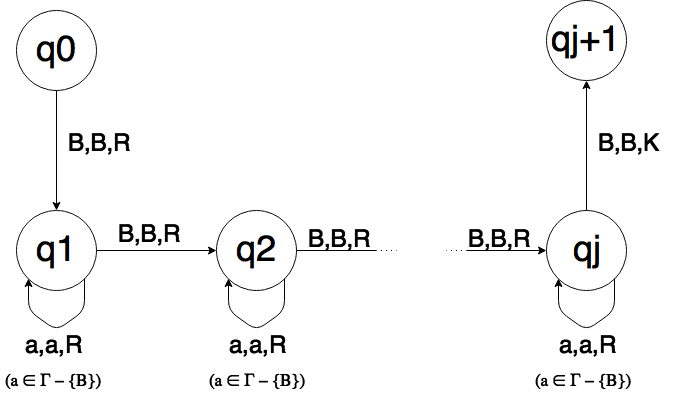
\includegraphics[scale=0.4]{graphics/figure_1.png}
        \end{figure}

        \PN Notar que:
    		\[
    		  \begin{array}{lcr}
            \alpha B \beta_{1} B \beta_{2} B \dotsc B \beta_{j} B \gamma &\overset{\ast}{\vdash}& \alpha B \beta_{1} B
              \beta_{2} B \dotsc B \beta_{j} B \gamma \\
            \ \ \uparrow && \uparrow \ \ \\
            \ \ q_{0} && q_{f} \ \
          \end{array}
    		\]

        \PN siempre que $\alpha, \gamma \in \Gamma ^{\ast}, \beta_{1}, \dotsc, \beta_{j} \in (\Gamma -\{B\})^{\ast}$.

      \item $I_{j}$ una máquina tal que:
    		\[
    		  \begin{array}{lcr}
            \alpha B \beta_{1} B
            \beta_{2} B \dotsc B \beta_{j} B \gamma &\overset{\ast}{\vdash}&  \alpha B \beta_{1} B \beta_{2} B \dotsc B
            \beta_{j} B \gamma \\
            \qquad\qquad\qquad\qquad \ \uparrow && \uparrow \qquad\qquad\qquad\qquad \ \\
            \qquad\qquad\qquad\qquad \ q_{0} && q_{f} \qquad\qquad\qquad\qquad \
          \end{array}
    		\]

        \PN siempre que $\alpha, \gamma \in \Gamma ^{\ast}, \beta_{1}, \dotsc, \beta_{j} \in (\Gamma -\{B\})^{\ast}$.

      \item $TD_{j}$ una máquina con un solo estado final $q_{f}$ y tal que:
    		\[
          \begin{array}{ccc}
            \alpha B \gamma &\overset{\ast}{\vdash} &\alpha B B \gamma \\
            \uparrow && \uparrow \ \ \\
            q_{0} & & q_{f} \ \
          \end{array}
        \]

        \PN cada vez que $\alpha, \gamma \in \Gamma^{\ast}$ y $\gamma$ tiene exactamente $j$ ocurrencias de $B$, es
        decir, la máquina $TD_{j}$ corre un espacio a la derecha todo el bloque $\gamma$ y agrega un blanco en el
        espacio que se genera a la izquierda de dicho bloque. Por ejemplo, para el caso de $\Sigma =\{\&\}$ podemos
        tomar $TD_{3}$ igual a la siguiente máquina:

        \begin{figure}[h]
          \centering
          \includegraphics[scale=0.4]{graphics/figure_3.png}
        \end{figure}

      \pagebreak
      \item $TI_{j}$ una máquina tal que:
    		\[
          \begin{array}{ccc}
            \alpha B \sigma \gamma &\overset{\ast}{\vdash}& \alpha B \gamma \\
            \uparrow \ && \uparrow \\
            q_{0} \ \ && q_{f}
          \end{array}
    	  \]

        \PN cada vez que $\alpha \in \Gamma ^{\ast }$, $\sigma \in \Gamma $ y $\gamma $ tiene exactamente $j$
        ocurrencias de $B$, es decir la máquina $TI_{j}$ corre un espacio a la izquierda todo el bloque $\gamma $ (por
        lo cual en el lugar de $\sigma $ queda el primer símbolo de $\gamma $).
    \end{itemize}

    \vspace{5mm}
    \PN Teniendo las máquinas auxiliares antes definidas podemos combinarlas para obtener las máquinas simuladoras de
    instrucciones. Por ejemplo $M_{i}^{a}$ puede ser la siguiente máquina:

    \begin{figure}[h]
      \centering
      \includegraphics[scale=0.4]{graphics/figure_4.png}
    \end{figure}

    \PN En la siguiente máquina, tenemos una posible forma de diseñar la máquina $IF_{i}^{a}$.

    \begin{figure}[h]
      \centering
      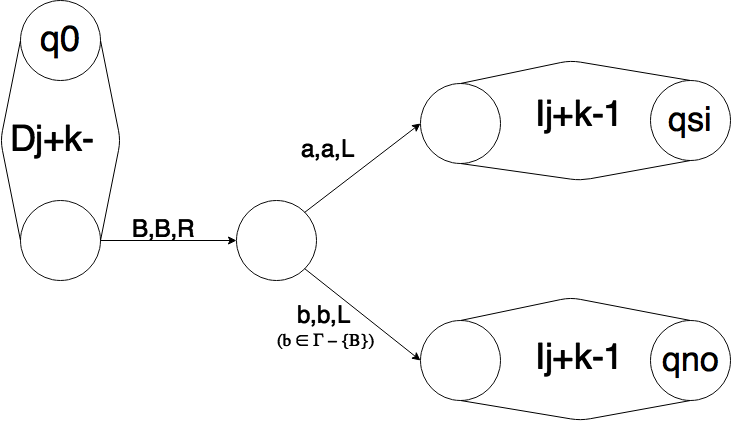
\includegraphics[scale=0.33]{graphics/figure_2.png}
    \end{figure}

    \pagebreak
    \PN En la siguiente máquina tenemos una posible forma de diseñar la máquina $M_{i\leftarrow j}^{\ast}$ para el caso
    $\Sigma = \{a,b\}$ y $i < j$:

    \begin{figure}[h]
      \centering
      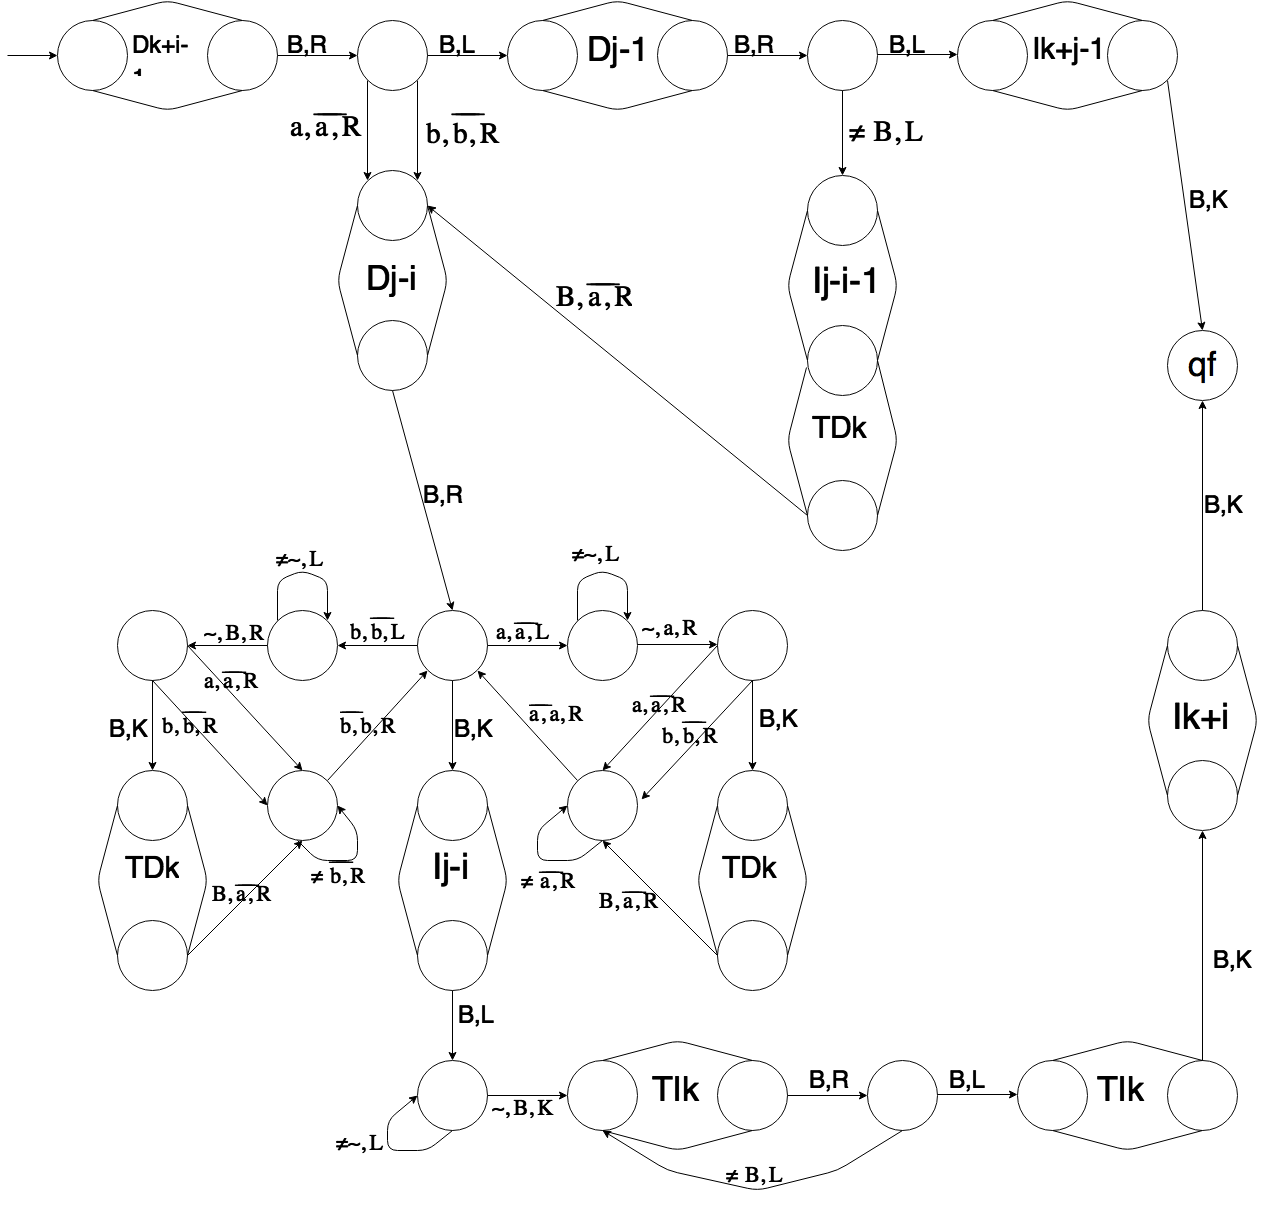
\includegraphics[scale=0.33]{graphics/figure_7.png}
    \end{figure}

    \pagebreak
    \PN Supongamos ahora que $\mathcal{P} = I_{1}, \dotsc, I_{n}$. Para cada $i = 1, \dotsc, n$, definiremos una máquina
    $M_{i}$ que simulará la instrucción $I_{i}$. Luego uniremos adecuadamente dichas máquinas para formar la máquina que
    simulará a $\mathcal{P}$.

		\begin{itemize}
			\item Si $Bas(I_{i})=\mathrm{N}\bar{j} \leftarrow \mathrm{N}\bar{j} + 1$ tomaremos $M_{i} = M_{j}^{+}$
	    \item Si $Bas(I_{i})=\mathrm{N}\bar{j} \leftarrow \mathrm{N}\bar{j} \dot{-} 1 $ tomaremos $M_{i} =
        M_{j}^{\dot{-}}$
	    \item Si $Bas(I_{i})=\mathrm{N}\bar{j} \leftarrow 0$ tomaremos $M_{i} = M_{j \leftarrow 0}$
	    \item Si $Bas(I_{i})=\mathrm{N}\bar{j} \leftarrow \mathrm{N}\bar{m}$ tomaremos $M_{i} = M_{j \leftarrow m}^{\#}$
	    \item Si $Bas(I_{i})=\mathrm{IF} \ \mathrm{N}\bar{j} \not = 0 \ \mathrm{GOTO} \ \mathrm{L}\bar{m}$ tomaremos
        $M_{i} = IF_{j}$
	    \item Si $Bas(I_{i})=\mathrm{P}\bar{j} \leftarrow \mathrm{P}\bar{j}.a$ tomaremos $M_{i}=M_{j}^{a}$
	    \item Si $Bas(I_{i})=\mathrm{P}\bar{j} \leftarrow \ ^{\curvearrowright} \mathrm{P}\bar{j}$ tomaremos $M_{i} =
        M_{j}^{\curvearrowright}$
	    \item Si $Bas(I_{i})=\mathrm{P}\bar{j} \leftarrow \varepsilon$ tomaremos $M_{i} = M_{j\leftarrow \varepsilon}$
	    \item Si $Bas(I_{i})=\mathrm{P}\bar{j} \leftarrow \mathrm{P}\bar{m}$ tomaremos $M_{i} = M_{j \leftarrow m}^{\ast}$
	    \item Si $Bas(I_{i})=\mathrm{IF} \ \mathrm{P}\bar{j} \ \mathrm{BEGINS} \ a \ \mathrm{GOTO} \ \mathrm{L}\bar{m}$
        tomaremos $M_{i} = IF_{j}^{a}$
	    \item Si $Bas(I_{i})=\mathrm{SKIP}$ tomaremos $M_{i} = M_{\mathrm{SKIP}}$.
	    \item Si $Bas(I_{i})=\mathrm{GOTO} \ \mathrm{L}\bar{m}$ tomaremos $M_{i} = M_{\mathrm{GOTO}}$
		\end{itemize}

    \PN Dado que la máquina $M_{i}$ puede tener uno o dos estados finales, se representará como se muestra en la
    siguiente figura:

    \begin{figure}[h]
      \centering
      \includegraphics[scale=0.4]{graphics/figure_5.png}
    \end{figure}

    \PN entendiendo que en el caso en que $M_{i}$ tiene un solo estado final, este esta representado por el circulo de
    abajo a la izquierda y en el caso en que $M_{i}$ tiene dos estados finales, el estado final corresponde al estado
    $q_{si}$ y el otro al estado $q_{no}$.

    \PN Para armar la máquina que simulará a $\mathcal{P}$, primero unimos las máquinas $M_{1}, \dotsc, M_{n}$ como lo
    muestra la siguiente figura:

    \begin{figure}[h]
      \centering
      \includegraphics[scale=0.5]{graphics/figure_6.png}
    \end{figure}

    \pagebreak
    \PN Luego para cada $i$ tal que $Bas(I_{i})$ es de la forma $\alpha \ \mathrm{GOTO} \ \mathrm{L}\bar{m}$, ligamos
    con una flecha de la forma:
		\[
      \underrightarrow{\qquad B,B,K \qquad}
		\]

    \vspace{5mm}
    \PN el estado final $q_{si}$ de la $M_{i}$ con el estado inicial de la $M_{h}$, donde $h$ es tal que $I_{h}$ es la
    primer instrucción que tiene label $\mathrm{L}\bar{m}$. Es intuitivamente claro que la máquina así obtenida cumple
    con lo requerido aunque una prueba formal de esto puede resultar extremadamente tediosa.
	\end{proof}

  \pagebreak
	% Theorem 85: Con prueba.
	\begin{theorem}
		\PN Si $f: D_{f} \subseteq \omega^{n} \times \Sigma^{\ast m} \rightarrow O$ es $\Sigma$-recursiva, entonces $f$ es
    $\Sigma$-Turing computable.
  \end{theorem}
  \begin{proof}
    \PN Dado que $f$ es $\Sigma$-computable, existe $\mathcal{P} \in \mathrm{Pro}^{\Sigma}$ el cual computa $f$. Se
    probará solamente el caso $O = \SIGMA$. Notar que cuando $\mathcal{P}$ termina, en el estado alcanzado, las
    variables numéricas tienen todas el valor $0$ y las alfabéticas distintas de $\mathrm{P}1$ todas el valor
    $\varepsilon$.

    \PN Sean:
    \begin{itemize}
      \item $M$ la máquina de Turing con unit dada por el \textbf{Lemma 84}, donde elegimos el número $k$ con la
        propiedad adicional de ser mayor que $n$ y $m$.

      \item $M_{1}$ una máquina tal que para cada $(\vec{x},\vec{\alpha}) \in \omega^{n} \times \Sigma^{\ast m}$
      	\[
          \left\lfloor q_{0} B \shortmid^{x_{1}} B \dotsc B \shortmid^{x_{n}} B \alpha_{1} B \dotsc B \alpha_{m} B
          \right\rfloor \overset{\ast}{\vdash}\left\lfloor q B \shortmid^{x_{1}} B \dotsc B \shortmid^{x_{n}}
          B^{k-n} B \alpha_{1} B \dotsc B \alpha_{m} B \right\rfloor
      	\]

        \PN donde $q_{0}$ es el estado inicial de $M_{1}$ y $q$ es un estado tal que $\delta(q,\sigma) =
        \emptyset$, para cada $\sigma$.

      \item $M_{2}$ una máquina tal que para cada $\alpha \in \SIGMA$
      	\[
          \left\lfloor q_{0} B^{k+1} \alpha \right\rfloor \overset{\ast}{\vdash} \left\lfloor q B \alpha
          \right\rfloor
      	\]

        \PN donde $q_{0}$ es el estado inicial de $M_{2}$ y $q$ es un estado tal que $\delta(q,\sigma) =
        \emptyset$, para cada $\sigma$.
    \end{itemize}

    \PN Notar que la concatenación de $M_{1}$, $M$ y $M_{2}$, en ese orden, produce una máquina de Turing la cual
    computa $f$.
	\end{proof}

  % Theorem 86: Nada.
  \begin{theorem}
    \PN Este teorema no se evalua.
  \end{theorem}


\begin{thebibliography}{X}
\bibitem{Baz} \textsc{Diego Vaggione},
<<Apunte de Clase, 2017>>,
\textit{FaMAF, UNC}.
\bibitem{Baz} \textsc{Agustín Curto},
<<Carpeta de Clase, 2017>>,
\textit{FaMAF, UNC}.
\end{thebibliography}

\vspace{\fill}
\begin{center}
Por favor, mejorá este documento en github

\includegraphics[width=1cm]{graphics/github.png} \\
https://github.com/acurto714/resumenLengForm
\end{center}
\end{document}
